\ifdefined\pdfvariable \pdfvariable minorversion=7 \else
    \ifdefined\pdfminorversion \pdfminorversion=7 \fi
\fi

\documentclass[10pt,aspectratio=43]{beamer}

\usetheme{Copenhagen}
\usecolortheme{default}

\usepackage[utf8]{inputenc}
\usepackage[T1]{fontenc}
\usepackage{amsmath,amssymb,amsthm,bm}
\usepackage{booktabs}
\usepackage{multirow}
\usepackage{graphicx}
\usepackage{dsfont}
\usepackage{hyperref}
\usepackage{array}
\usepackage{xcolor}
\usepackage{tikz}

\setbeamertemplate{caption}[numbered]
\setbeamertemplate{navigation symbols}{}
\setbeamertemplate{headline}{}
\setbeamertemplate{page number in head/foot}[totalframenumber]

\setbeamercolor{author in head/foot}{fg=white,bg=black}
\setbeamercolor{title in head/foot}{fg=white,bg=structure.fg}

\setbeamerfont{author in head/foot}{size=\scriptsize}
\setbeamerfont{title in head/foot}{size=\scriptsize}

\makeatletter
\def\viva@progressdot#1/#2\relax{%
    \begin{tikzpicture}[baseline=-0.5ex]
        \path[use as bounding box] (0pt,-2pt) rectangle (5pt,2pt);
        \ifnum\c@page<#1\relax
            \draw[white!55!black,line width=0.4pt]
            (2.5pt,0pt) circle[radius=1.4pt];
        \else
            \ifnum\c@page>#2\relax
                \fill[white!70!black] (2.5pt,0pt) circle[radius=1.4pt];
            \else
                \fill[white] (2.5pt,0pt) circle[radius=1.9pt];
            \fi
        \fi
    \end{tikzpicture}%
}
\newcommand{\vivasectiondots}{%
    \ifbeamer@inappendix\else
        \begingroup
        \def\sectionentry##1##2##3##4##5{}%
        \def\slideentry##1##2##3##4##5##6{%
            \ifnum##6=\c@part\relax
                \ifnum##1=\c@section\relax
                    \ifnum##1>0\relax
                        \beamer@link(##4){\viva@progressdot##4\relax}%
                    \fi
                \fi
            \fi
        }%
        \dohead
        \endgroup
    \fi
}
\makeatother

\setbeamertemplate{footline}{%
    \leavevmode%
    \hbox{%
        \begin{beamercolorbox}[
                wd=.28\paperwidth,ht=3.6ex,dp=1.8ex,center
            ]{author in head/foot}%
            \usebeamerfont{author in head/foot}\insertshortauthor
        \end{beamercolorbox}%
        \begin{beamercolorbox}[
                wd=.72\paperwidth,ht=3.6ex,dp=1.8ex
            ]{title in head/foot}%
            \usebeamerfont{title in head/foot}%
            \makebox[.20\paperwidth][c]{\insertshorttitle}%
            \makebox[.16\paperwidth][c]{\insertsectionhead}%
            \makebox[.28\paperwidth][c]{\vivasectiondots}%
            \makebox[.08\paperwidth][c]{\insertframenumber/\inserttotalframenumber}%
        \end{beamercolorbox}%
    }%
    \vskip0pt%
}

\usebeamercolor{structure}
\colorlet{vivatag}{structure.fg}
\newcommand{\ourstext}{Original contribution}

\newif\ifvivaours
\newcommand{\ours}{\global\vivaourstrue}

\newsavebox{\vivatagbox}
\newlength{\vivatagwidth}
\newlength{\vivatagspace}
\newlength{\vivatagdrop}
\setlength{\vivatagdrop}{11.8pt}
\AtBeginDocument{%
    \savebox{\vivatagbox}{\small\bfseries\ourstext}%
    \setlength{\vivatagwidth}{\dimexpr\wd\vivatagbox + 0.95cm\relax}%
}
\setbeamertemplate{frametitle}[default][left,rightskip=\vivatagspace]

\addtobeamertemplate{frametitle}{%
    \ifvivaours
        \setlength{\vivatagspace}{\vivatagwidth}%
    \else
        \setlength{\vivatagspace}{0pt}%
    \fi
}{%
    \ifvivaours
        \begin{tikzpicture}[remember picture, overlay]
            \path (0,0) -- (current page.north) coordinate[midway] (vivamid);
            \node[anchor=east, xshift=-0.26cm, yshift=0.5\vivatagdrop, rounded corners=2pt,
                fill=white, text=vivatag, inner xsep=5pt, inner ysep=2pt,
                font=\small\bfseries]
            at (current page.east |- vivamid) {\ourstext};
        \end{tikzpicture}%
        \vspace{-\vivatagdrop}%
        \global\vivaoursfalse
    \fi
}

\title[SelVAEGen]{Selective protein-targeted drug generation}
\author{Iago Riveiro Santos Dutra}
\date{}

\begin{document}

\begin{frame}[plain]
    \titlepage
    \vspace{-2.5cm}
    \begin{center}
        \small
        Supervisor: Prof. Alberto Paccanaro

        \vspace{0.5cm}
        Escola de Matemática Aplicada

        Fundação Getúlio Vargas
    \end{center}

    \vfill

    \begin{center}
        September 21\textsuperscript{st}, 2026
    \end{center}

    \vspace{-1cm}
\end{frame}

\section{Introduction}
\begin{frame}{Introduction}
    \begin{figure}[h]
        \centering
        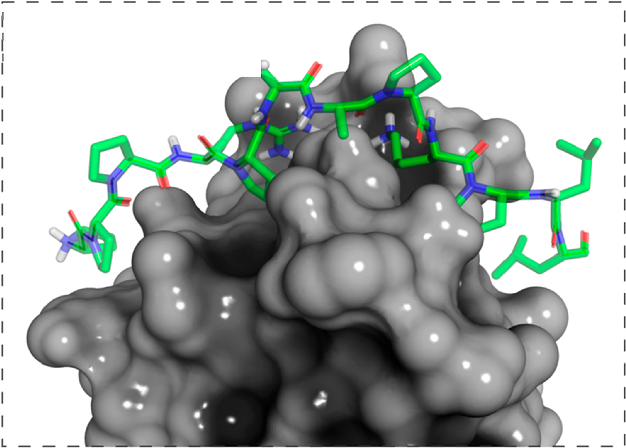
\includegraphics[width=0.8\textwidth]{figs/chapters/1.pdf}
    \end{figure}
\end{frame}

\begin{frame}{Example}
    \begin{figure}[h]
        \centering
        
\includegraphics[width=\textwidth]{figs/barbie.png}
    \end{figure}

    \vfill
    \centering
    Melanotan-II tans you! No Sun involved!

    \vfill
\end{frame}

\begin{frame}{Example}
    \begin{figure}[h]
        \centering
        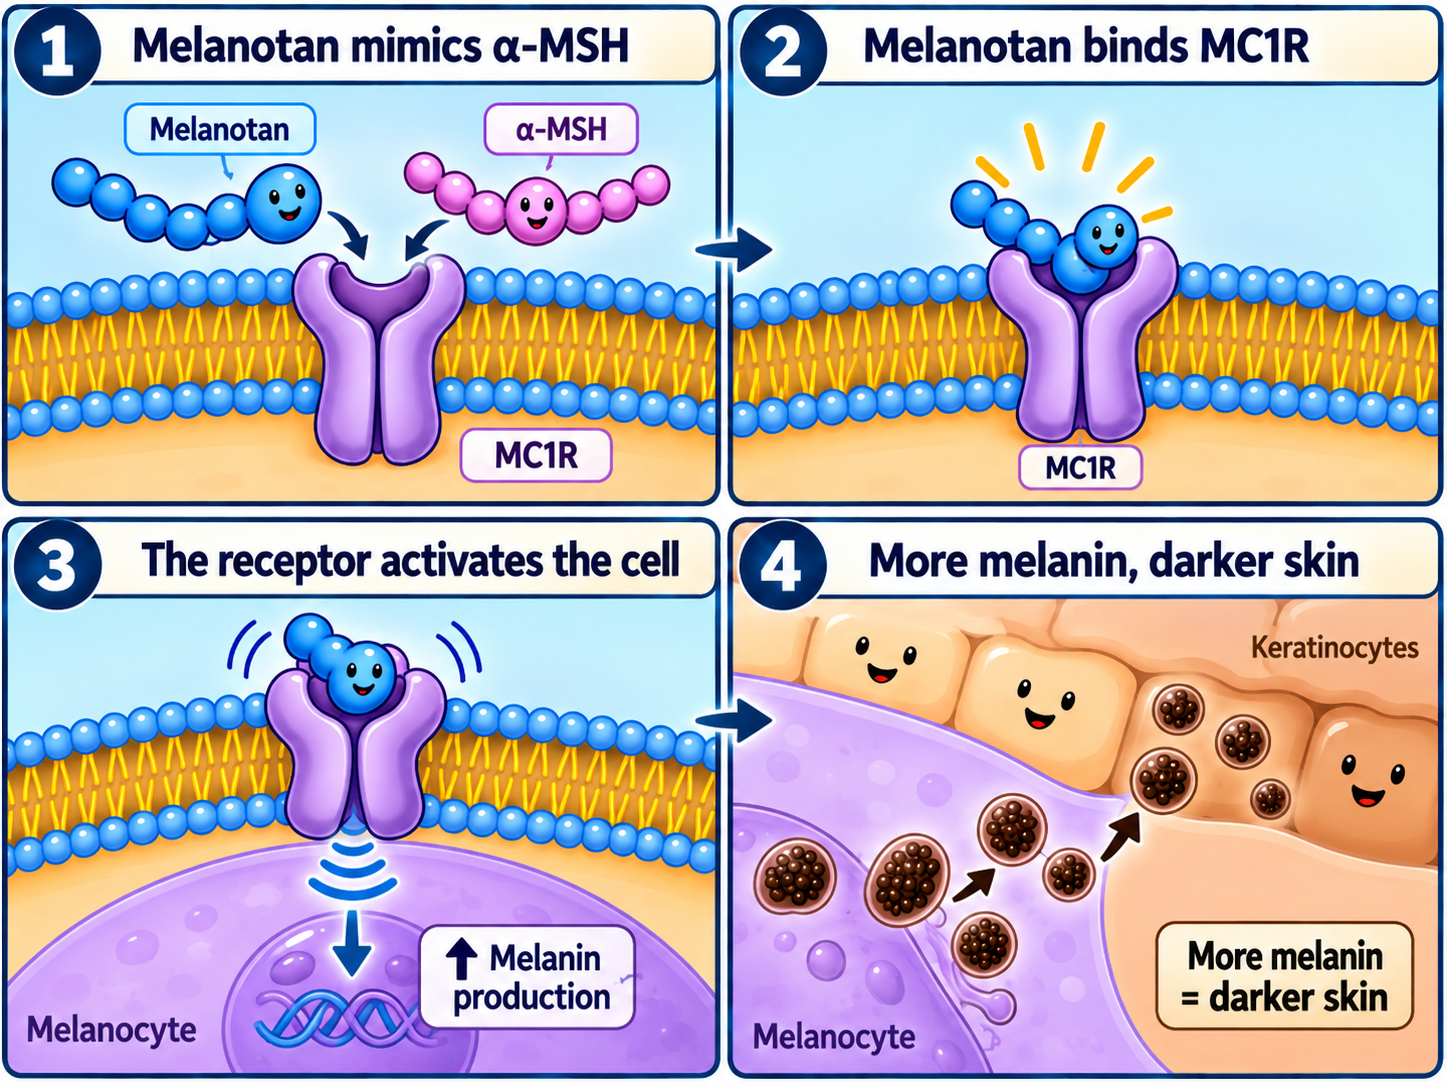
\includegraphics[width=0.9\textwidth]{figs/comic.png}
    \end{figure}
\end{frame}

\begin{frame}{Except...}
    It was made for MC1R. It also binds to MC3R and MC4R.

    \medskip
    \begin{itemize}
        \item Nausea, vomiting, loss of appetite
        \item Priapism: painful erections lasting hours
        \item New and darkening moles, and reported cases of melanoma
    \end{itemize}

    \vfill
    \centering
    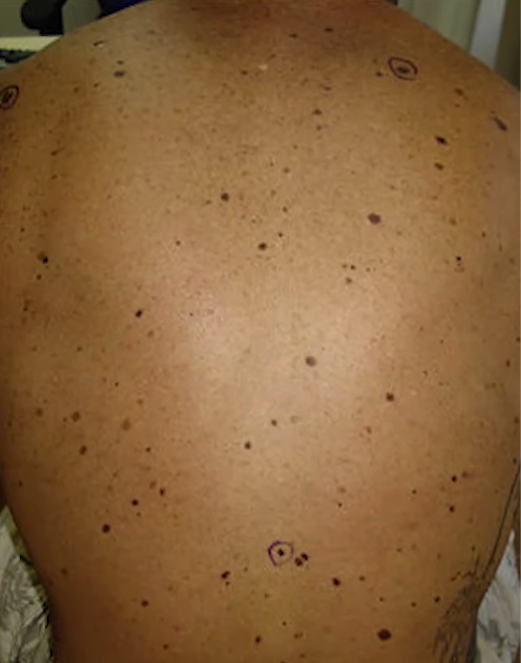
\includegraphics[height=0.40\textheight]{figs/cancer.png}%
    \hspace{0.8cm}%
    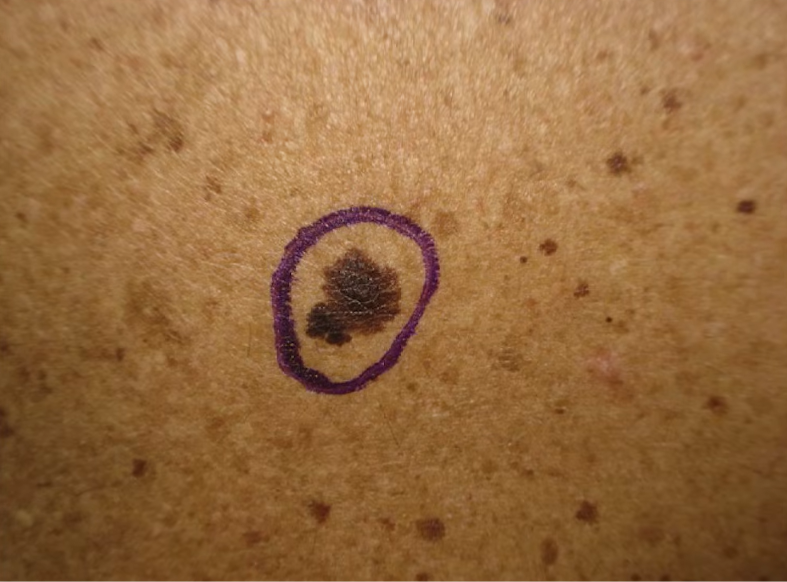
\includegraphics[height=0.40\textheight]{figs/cancer2.png}
    \vfill
\end{frame}

\section{Background}
\newcommand{\pastage}[2]{%
    \hangindent=1.5em
    \hangafter=1
    \textcolor{gray}{\textbf{#1}}\quad #2\par
    \vspace{0.15em}
}

\newcommand{\stage}[2]{%
    \hangindent=1.5em
    \hangafter=1
    \textbf{#1}\quad #2\par
    \vspace{0.15em}
}

\begin{frame}{What has been done}
    \centering
    \makebox[\textwidth][c]{%
        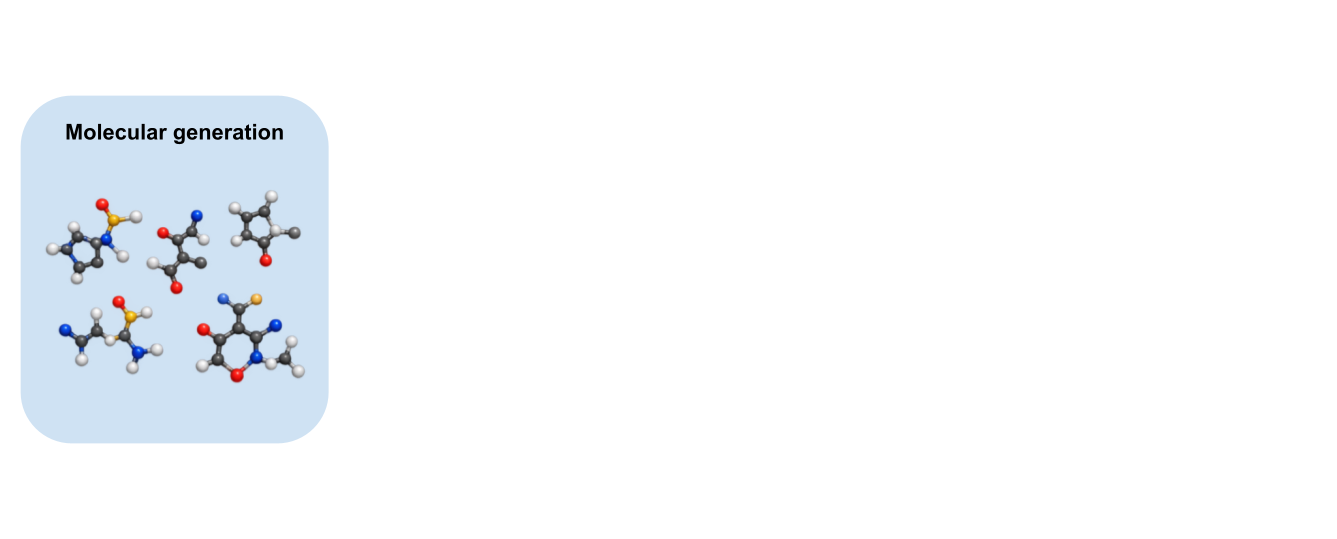
\includegraphics[width=1.04\textwidth]{figs/lit_a.png}%
    }

    \vspace{0.6em}
    \footnotesize\raggedright
    \stage{Molecular generation}{[Kingma \& Welling, \emph{ICLR} 2014] \quad
        \mbox{[G\'omez-Bombarelli \emph{et al.}, \emph{ACS Cent. Sci.} 2018]} \quad
        [Brown \emph{et al.}, \emph{JCIM} 2019]}
\end{frame}

\begin{frame}{What has been done}
    \centering
    \makebox[\textwidth][c]{%
        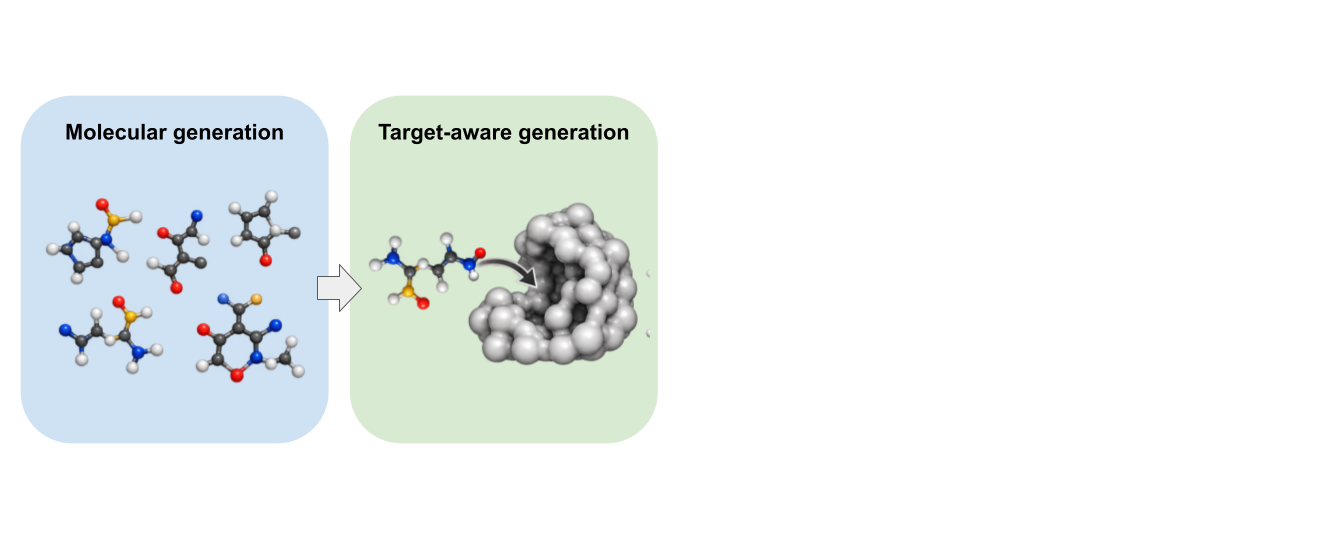
\includegraphics[width=1.04\textwidth]{figs/lit_b.png}%
    }

    \vspace{0.6em}
    \footnotesize\raggedright
    \pastage{Molecular generation}{\textcolor{gray}{[Kingma \& Welling 2014] \quad
            [G\'omez-Bombarelli \emph{et al.} 2018] \quad [Brown \emph{et al.} 2019]}}
    \stage{Target-aware generation}{[Sohn \emph{et al.}, \emph{NeurIPS} 2015] \quad
        \mbox{[Uludo\u gan \emph{et al.}, \emph{Bioinformatics} 2022]}\quad
        [Chen \emph{et al.} 2023]}
\end{frame}

\begin{frame}{What has been done}
    \centering
    \makebox[\textwidth][c]{%
        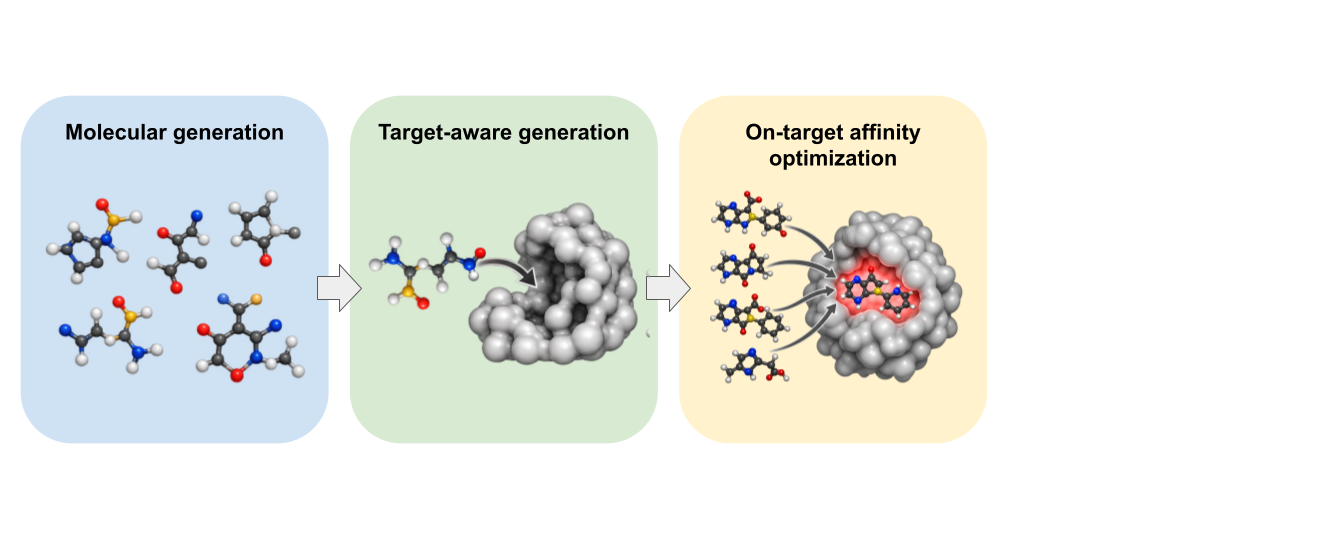
\includegraphics[width=1.04\textwidth]{figs/lit_c.png}%
    }

    \vspace{0.6em}
    \footnotesize\raggedright
    \pastage{Molecular generation}{\textcolor{gray}{[Kingma \& Welling 2014] \quad
            [G\'omez-Bombarelli \emph{et al.} 2018] \quad [Brown \emph{et al.} 2019]}}
    \pastage{Target-aware generation}{\textcolor{gray}{[Sohn \emph{et al.} 2015] \quad
            [Uludo\u gan \emph{et al.} 2022] \quad \mbox{[Chen \emph{et al.} 2023]}}}
    \stage{On-target affinity optimization}{[Shah \emph{et al.} 2025 (DeepDTAGen)] \quad
        \mbox{[Creanza \emph{et al.} 2025 (Prot2Drug)]} \quad
        [Chen \emph{et al.} 2025 (ZeroGEN)]}
\end{frame}

\begin{frame}{What has been done}
    \centering
    \makebox[\textwidth][c]{%
        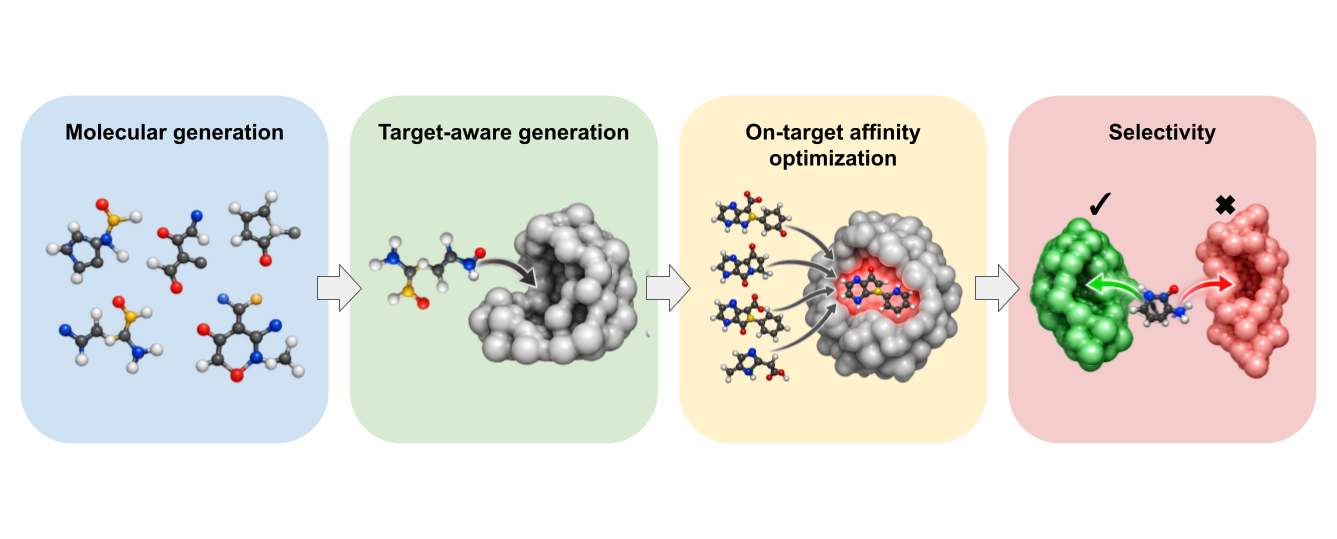
\includegraphics[width=1.04\textwidth]{figs/lit_d.png}%
    }

    \vspace{0.6em}
    \footnotesize\raggedright
    \pastage{Molecular generation}{\textcolor{gray}{[Kingma \& Welling 2014] \quad
            [G\'omez-Bombarelli \emph{et al.} 2018] \quad [Brown \emph{et al.} 2019]}}
    \pastage{Target-aware generation}{\textcolor{gray}{[Sohn \emph{et al.} 2015] \quad
            [Uludo\u gan \emph{et al.} 2022] \quad \mbox{[Chen \emph{et al.} 2023]}}}
    \pastage{On-target affinity optimization}{\textcolor{gray}{[Shah \emph{et al.} 2025] \quad
            [Creanza \emph{et al.} 2025] \quad \mbox{[Chen \emph{et al.} 2025]}}}
    \stage{Selectivity}{[Chenthamarakshan \emph{et al.} 2020 (CogMol)] \quad
        [Gao \emph{et al.} 2024 ($\Delta$ score)] \quad [Zou \emph{et al.} 2025] \quad
        [Koban \emph{et al.} 2026 (ConGen)] \quad [Qin \emph{et al.} 2026 (DBMol)]}
\end{frame}

\section{Metrics}
\begin{frame}[t]{On notation}
    We train a generator $G_\omega$

    \medskip
    \hspace*{1cm}\textbf{Input:} a target protein $p_i$

    \medskip
    \hspace*{1cm}\textbf{Output:} $K$ candidate drugs sampled independently:
    \[
    d_{i,1},\ldots,d_{i,K}
    \overset{\mathrm{iid}}{\sim} G_\omega(\,\cdot\mid p_i)
    \]

    \vfill

    \begin{figure}[h]
        \centering
        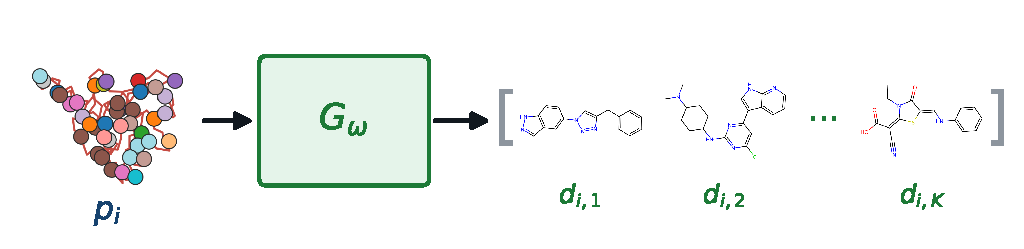
\includegraphics[width=\textwidth]{figs/notation_generator.pdf}
    \end{figure}

    \vfill
\end{frame}

\begin{frame}[t]{On notation}
    We train a generator model $G_\omega$

    \medskip
    We have a pre-trained ``oracle'' $f_\theta$

    \medskip
    \hspace*{1cm}\textbf{Input:} a drug-protein pair $(d_{i,k},\ p_j)$

    \medskip
    \hspace*{1cm}\textbf{Output:} their estimated binding affinity:

    \medskip
    \centering
    $A_{i,k}^{(j)}=f_\theta(d_{i,k},\ p_j)$

    \begin{figure}[h]
        \centering
        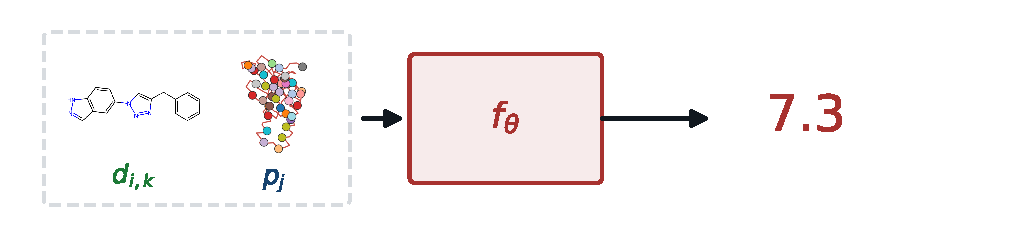
\includegraphics[width=\textwidth]{figs/notation_oracle.pdf}
    \end{figure}
\end{frame}

\begin{frame}[t]{On notation}
    We train a generator model $G_\omega$

    \medskip
    We have a pre-trained ``oracle'' $f_\theta$

    \medskip
    We evaluate every drug against every protein

    \medskip
    \hspace*{1cm}$\mathcal{A}_{\mathrm{on}}=\left\{A_{i,k}^{(i)} \; \; \forall\ i,k \right\} \sim p_G$

    \medskip
    \hspace*{1cm}$\mathcal{A}_{\mathrm{off}}=\left\{A_{i,k}^{(j)} \; \; \forall \ i,j,k;\;j\neq i \right\} \sim q_G$

    \begin{figure}[h]
        \centering
        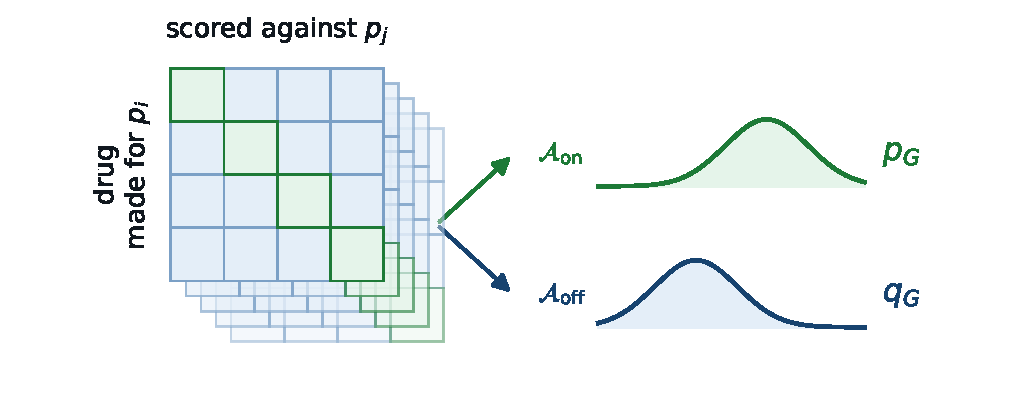
\includegraphics[width=\textwidth]{figs/notation_sets.pdf}
    \end{figure}
\end{frame}

\begin{frame}[c]{Thresholds}
    Each dataset has an affinity threshold.

    \bigskip

    \centering
    \renewcommand{\arraystretch}{1.8}

    \resizebox{\textwidth}{!}{%
        \begin{tabular}{
                >{\color{black}}l
                >{\color{black!20}}r
                >{\color{black!20}}r
                >{\color{black!20}}r
                >{\color{black!20}}r
                >{\color{black}}r
                >{\color{black!20}}r
            }
            \toprule
            \textbf{Dataset} &
            \textbf{Drugs} &
            \textbf{Proteins} &
            \textbf{Records} &
            \textbf{Density (\%)} &
            \textbf{Threshold} &
            \textbf{Positive (\%)} \\
            \midrule

            KIBA      & 2,015  & 225   & 115,822 & 25.55  & 12.10 & 20.86 \\
            Davis     & 64     & 427   & 27,328  & 100.00 & 7.00  & 8.03  \\
            BindingDB & 31,053 & 1,200 & 77,412  & 0.21   & 7.00  & 30.43 \\
            Papyrus   & 81,147 & 749   & 239,226 & 0.39   & 7.00  & 32.15 \\

            \bottomrule
        \end{tabular}}

\end{frame}

\newcommand{\blindspot}[1]{%
    \vfill
    {\color{red!55!black}\textbf{Blind spot:} #1}
    \vspace{0.3em}}

\ours
\begin{frame}[t]{Utility}
    We start from a simple notion.

    $$U(G_\omega, \tau) = \mathbb{P}_{p_G}(X \geq \tau) - \mathbb{P}_{q_G}(X \geq \tau)$$

    \vfill
    \centering
    \makebox[\textwidth][c]{%
        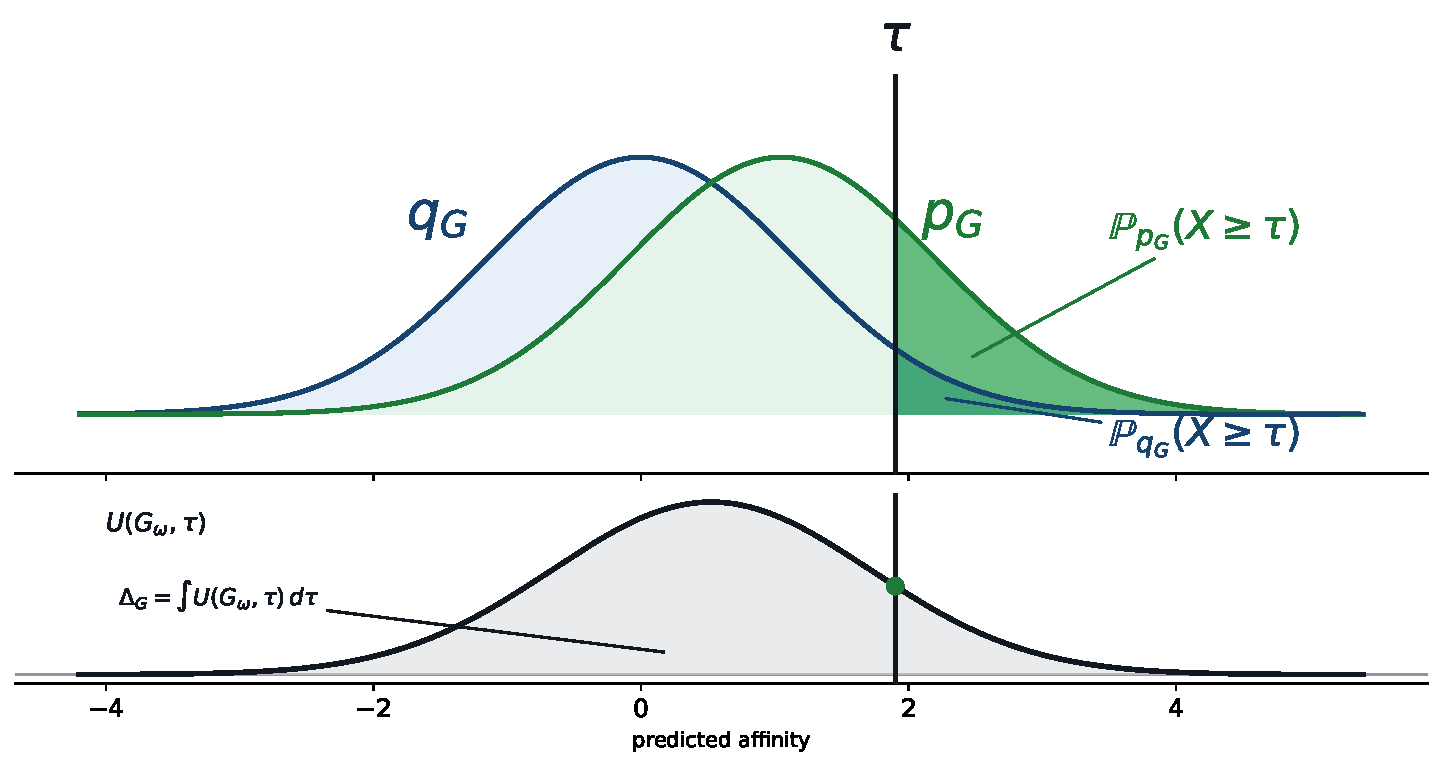
\includegraphics[width=1.10\textwidth, trim=0bp 135bp 0bp 0bp, clip]
        {figs/chapters/metrics.pdf}%
    }
\end{frame}

\begin{frame}[t]{Delta score}
    How much more a drug binds its own target than the rest.

    $$\delta(d_{i,k}) = A_{i,k}^{(i)} - \frac{1}{N-1}\sum_{j \neq i} A_{i,k}^{(j)},
    \qquad
    \Delta = \frac{1}{NK}\sum_{i=1}^{N}\sum_{k=1}^{K}\delta(d_{i,k})$$

    \vfill
    \centering
    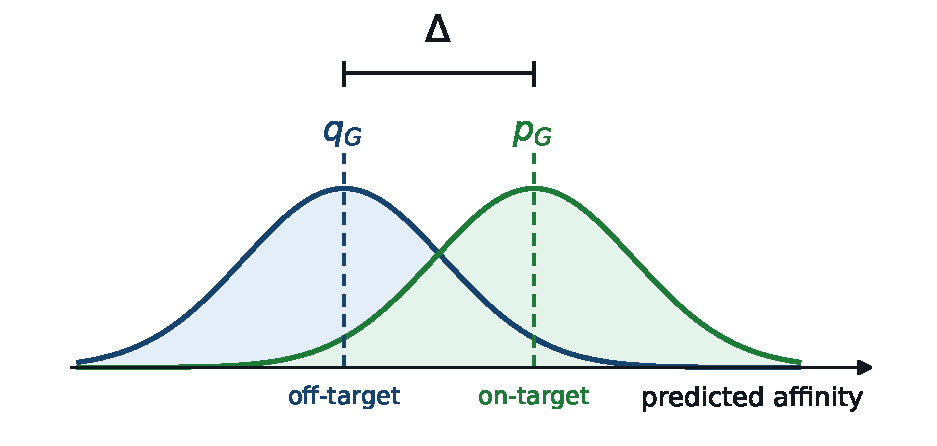
\includegraphics[width=0.92\textwidth]{figs/talk/metric_delta.pdf}
    \vfill

    \raggedright
    [Gao \emph{et al.} 2024 - Non-peer-reviewed arXiv preprint]
\end{frame}

\ours
\begin{frame}[t]{Distributional delta}
    Compare the whole distributions, not just their means.

    $$\mathrm{Dist.}\,\Delta = \mathrm{sign}\!\left(\mathbb{E}[p_G] - \mathbb{E}[q_G]\right)\,
    D_{\mathrm{KL}}\!\left(p_G \,\|\, q_G\right)$$

    \vfill
    \centering
    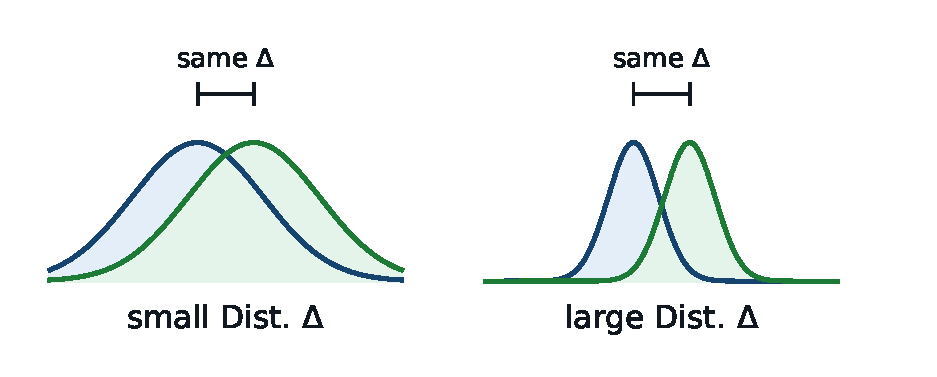
\includegraphics[width=0.92\textwidth]{figs/talk/metric_distributional.pdf}
    \vfill
\end{frame}

\ours
\begin{frame}[t]{Effective delta}
    Count only the drugs that matter.

    $$S = \left\{\, d_{i,k} \;:\; \text{valid, unique, novel, and } A_{i,k}^{(i)} \geq \tau
    \,\right\}$$

    $$\mathrm{Eff.}\,\Delta = \frac{1}{NK}\sum_{i=1}^{N}\sum_{k=1}^{K}
    \delta(d_{i,k}) \cdot \mathds{1}\!\left[d_{i,k} \in S\right]$$

    \vfill
    \centering
    \makebox[\textwidth][c]{%
        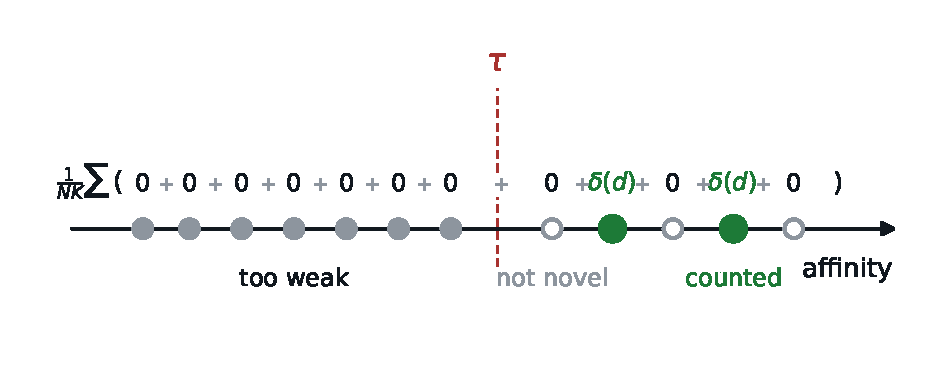
\includegraphics[width=1.10\textwidth]{figs/talk/metric_effective.pdf}%
    }
    \vfill
\end{frame}

\ours
\begin{frame}[t]{Directional consistency}
    In what fraction of individual comparisons is the on-target affinity actually the
    higher one?

    $$m(i) = \frac{1}{K(N-1)}\sum_{k=1}^{K}\sum_{j \neq i}
    \mathds{1}\!\left(A_{i,k}^{(i)} > A_{i,k}^{(j)}\right),
    \qquad
    \mathrm{Dir.Cons.} = \frac{1}{N}\sum_{i=1}^{N} m(i)$$

    \vfill
    \centering
    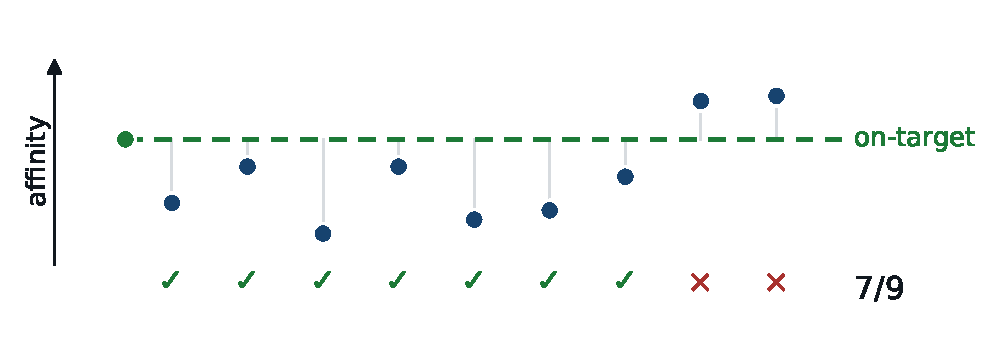
\includegraphics[width=0.92\textwidth]{figs/talk/metric_directional.pdf}
\end{frame}

\ours
\begin{frame}[t]{Tanimoto gap}
    Does the protein actually change which molecules come out?

    $$\mathrm{Gap} = \frac{1}{N}\sum_{i=1}^{N}
    \big[\, \underbrace{g_{\mathrm{within}}(i)}_{\substack{\text{similarity between two}\\
                \text{drugs made for } p_i}} \;-\;
        \underbrace{g_{\mathrm{cross}}(i)}_{\substack{\text{similarity to drugs}\\
                \text{made for other proteins}}} \,\big]$$

    \vfill
    \centering
    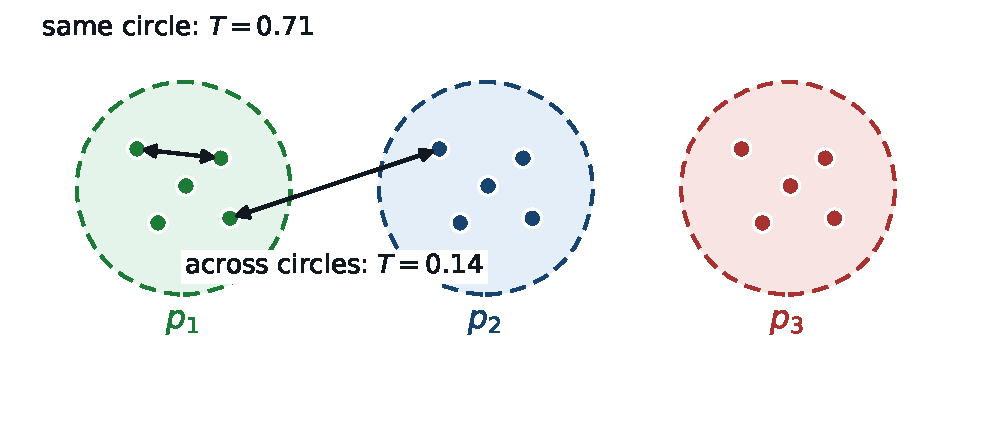
\includegraphics[width=0.86\textwidth]{figs/talk/metric_tanimoto.pdf}
    \vfill

    \raggedright
    Looks at structures rather than affinities.
\end{frame}

\begin{frame}[c]{State-of-the-art models are not selective}
    \centering
    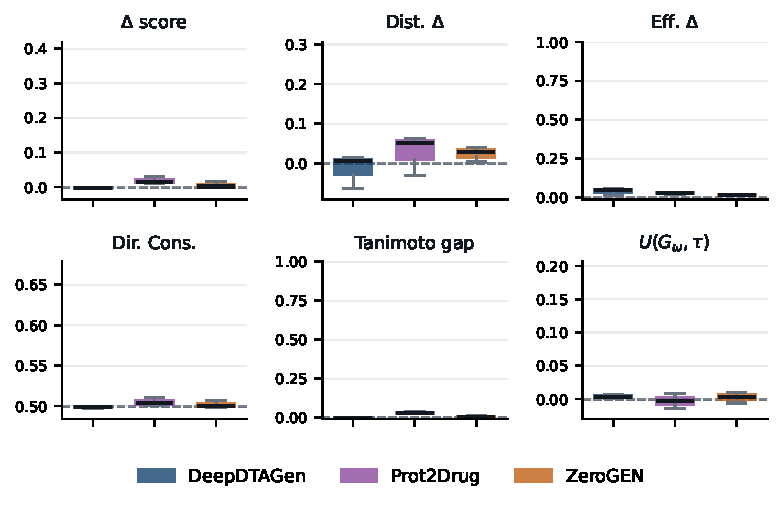
\includegraphics[width=\textwidth,height=0.7\textheight,keepaspectratio]
    {figs/talk/competitors_kiba.pdf}

    \raggedright
    DeepDTAGen: Nature Communications, 2025

    Prot2Drug: Journal of Chemical Information and Modeling, 2025

    ZeroGEN: Bioinformatics, 2025
\end{frame}

\section{Methods}

\ours
\begin{frame}[t]{Proteins define Gaussians}
    $$p(z \mid p_i) = \mathcal{N}\!\left(m_\psi(p_i),\ I\right)$$

    \vfill
    \centering
    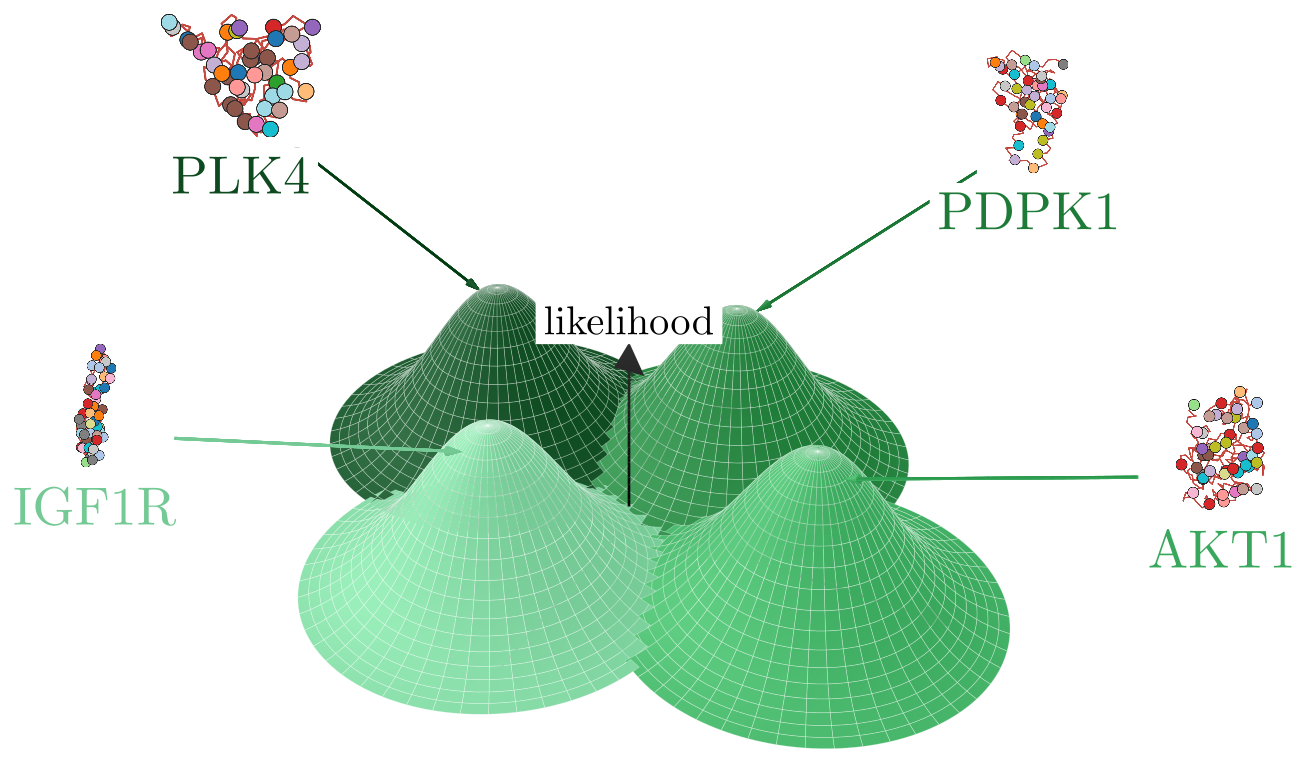
\includegraphics[height=0.70\textheight]{figs/talk/protein_field.png}

\end{frame}

\ours
\begin{frame}[t]{Drugs become Gaussians}
    $$q(z \mid d) = \mathcal{N}\!\left(\mu_d,\ \mathrm{diag}(\sigma_d^2)\right)$$

    \vfill
    \centering
    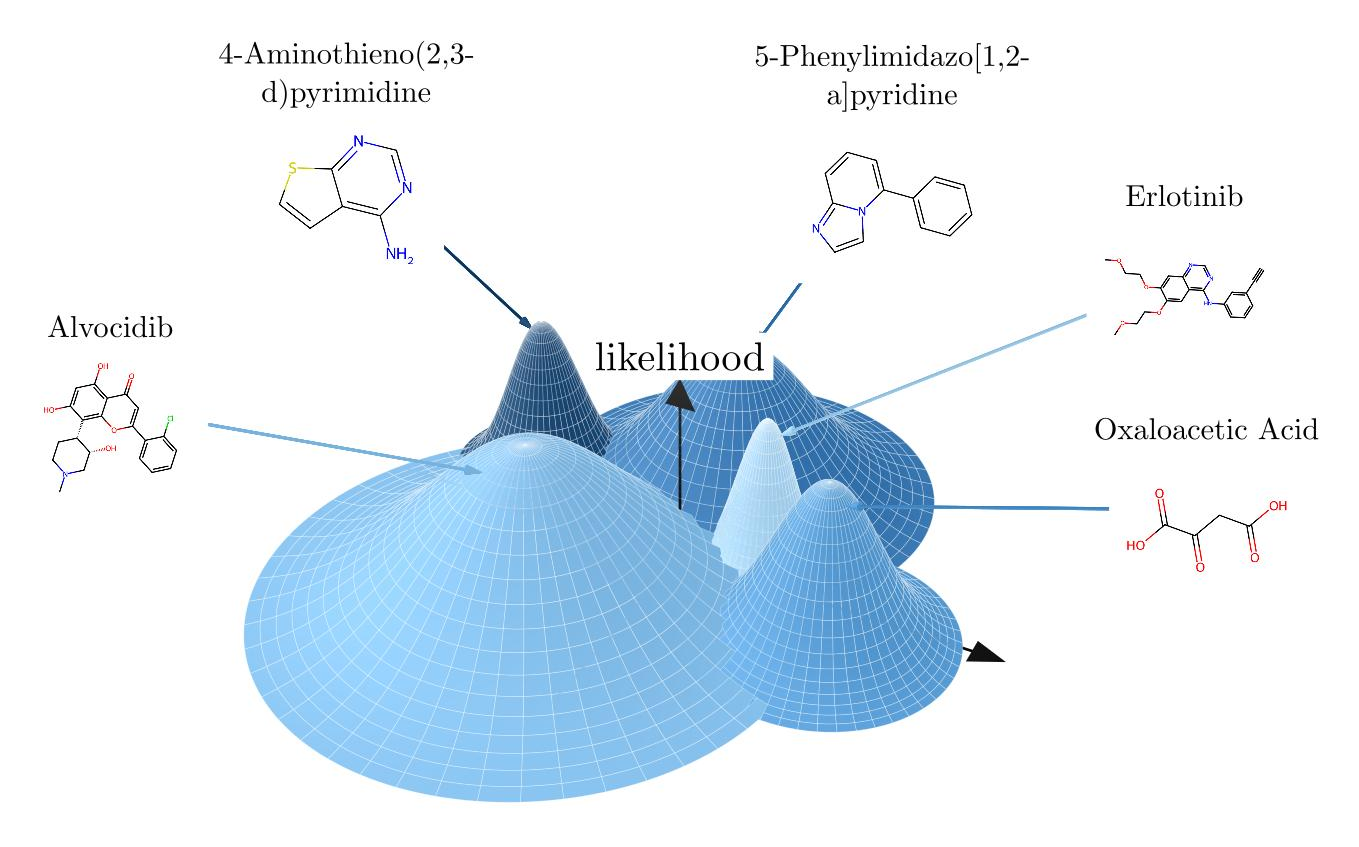
\includegraphics[height=0.7\textheight]{figs/chapters/methods.pdf}

\end{frame}

\ours
\begin{frame}[t]{Shared latent space}
    A drug is compatible with a protein if it has high likelihood under its distribution, and vice-versa.

    $$s(d, p) = -\tfrac{1}{2}\left\|\mu_d - m_\psi(p)\right\|_2^{2}$$

    \centering
    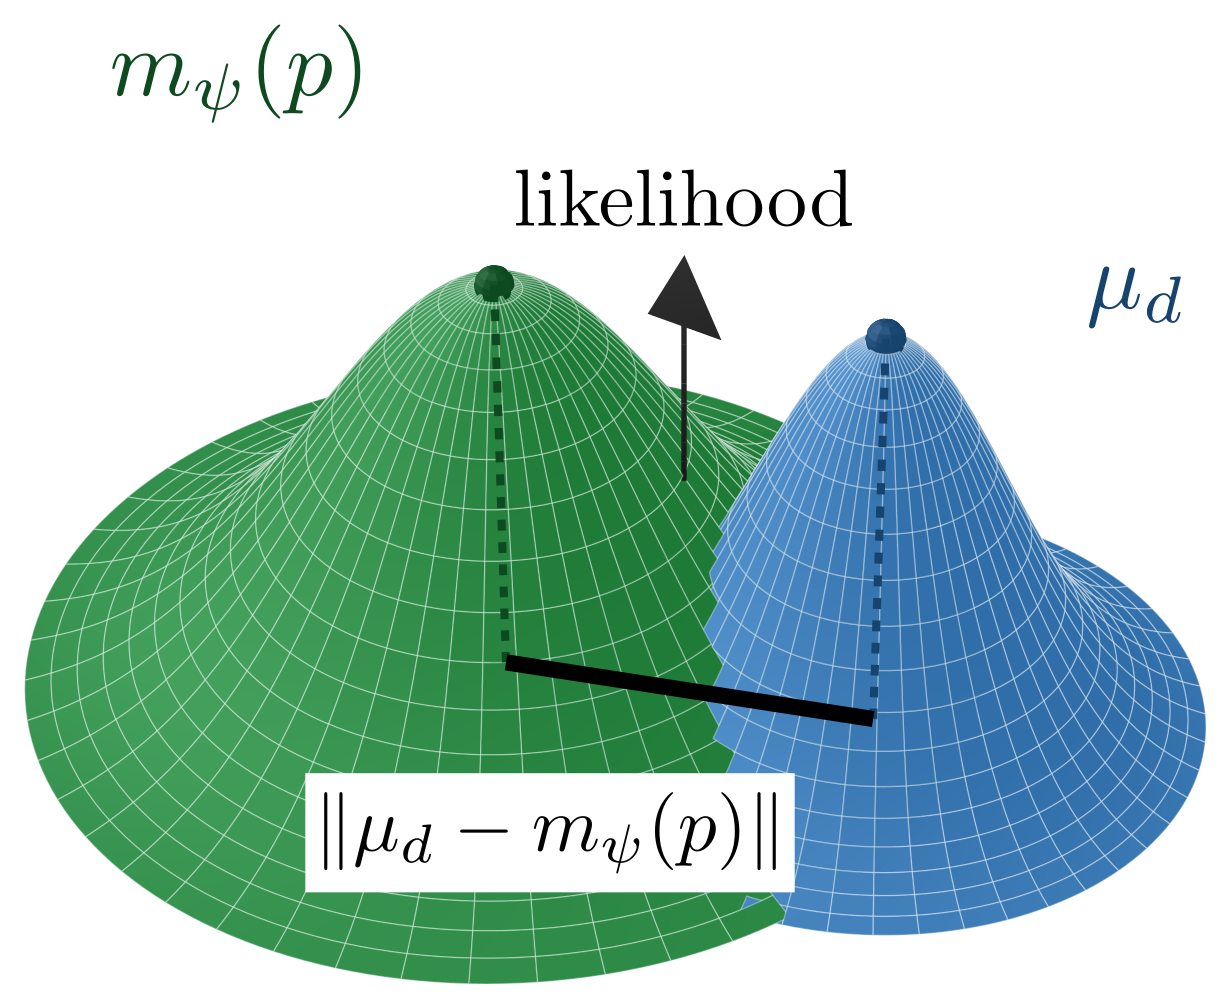
\includegraphics[height=0.5\textheight]{figs/talk/same_map.png}

    \raggedright
    \vspace{-0.75cm}
    \begin{align*}
        \Longrightarrow \text{Organize the geometry so that } &
        \text{\textbf{compatible} pairs are \textbf{close} and}\\
        &\text{\textbf{incompatible} pairs are \textbf{far} apart.}
    \end{align*}
    \vspace{-0.5cm}
\end{frame}

\ours
\begin{frame}{Our model}

    Selective Variational Auto-Encoder Generator (SelVAEGen)
    \vfill
    {
        \centering
        \makebox[\textwidth][c]{%
            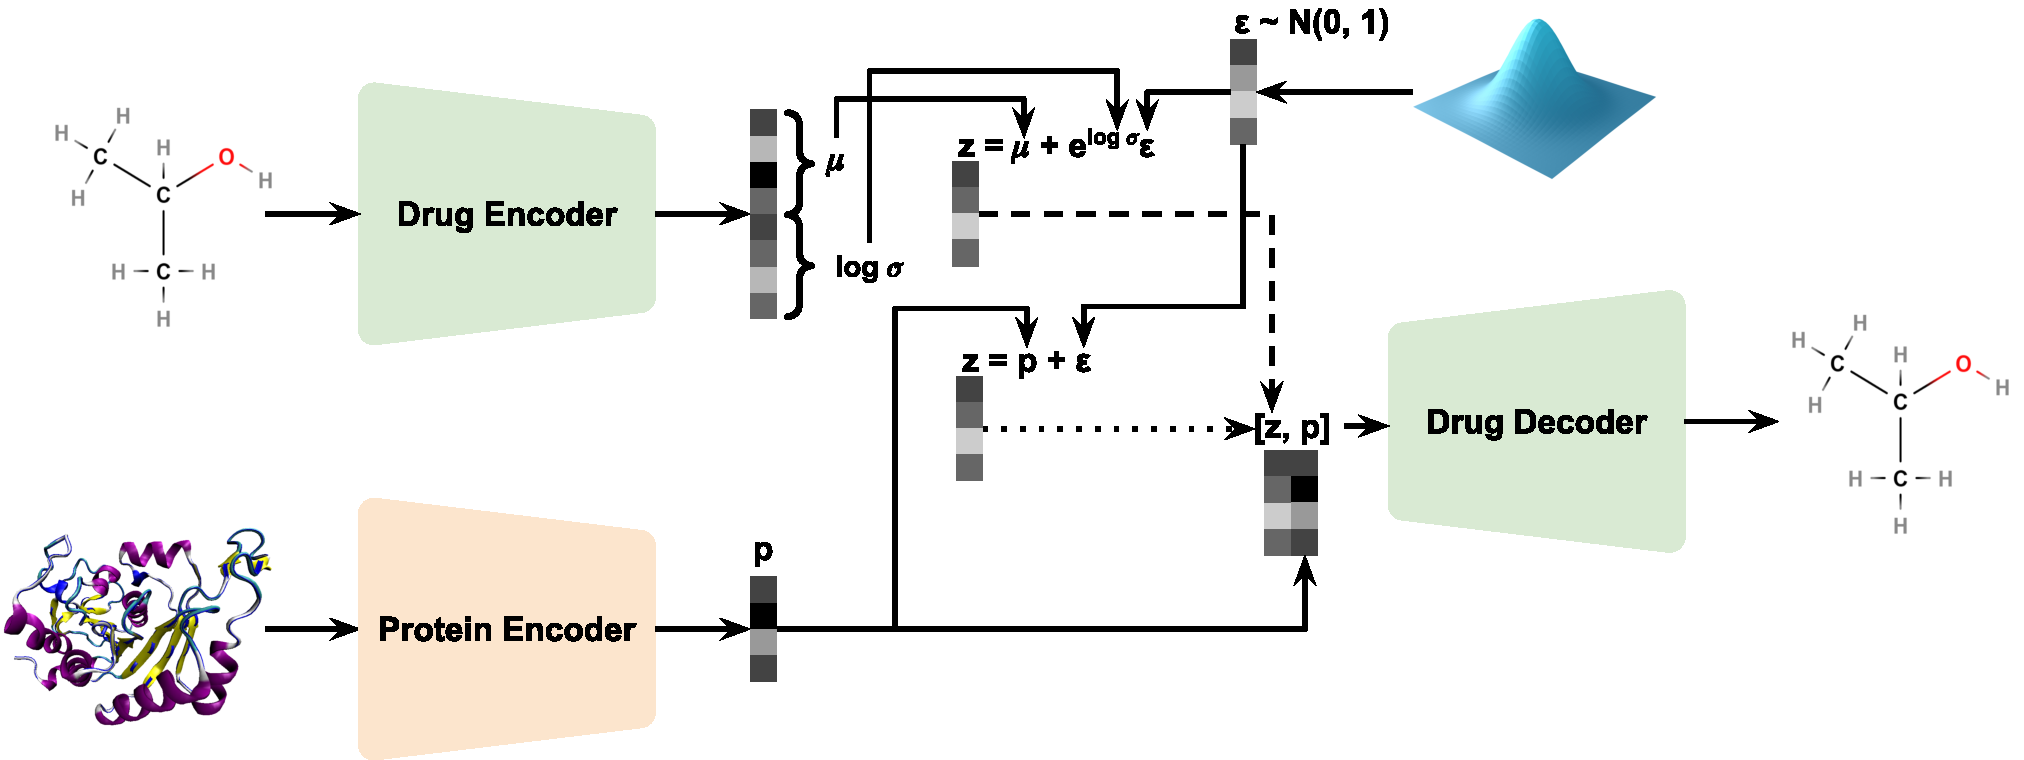
\includegraphics[width=1.15\textwidth]{figs/model/model.pdf}
        }
    }
    \vfill

    Drugs and proteins share a latent space in $\mathbb{R}^{128}$
\end{frame}

\ours
\begin{frame}{SelVAEGen}
    \begin{figure}[h]
        \centering
        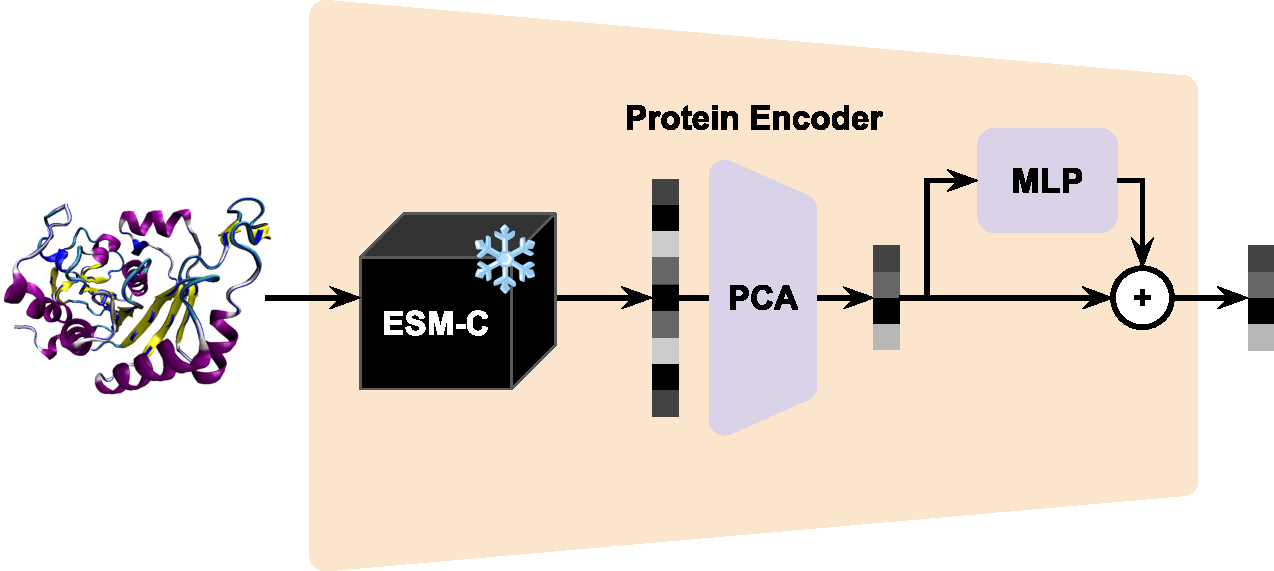
\includegraphics[width=\textwidth]{figs/model/protein_encoder.pdf}
    \end{figure}

    ESM-C makes per-amino-acid embeddings in $\mathbb{R}^{L\times 1152}$

    \vspace{0.2cm}

    We aggregate and reduce to $m_\psi(p)\in\mathbb{R}^{128}$

    \begin{tikzpicture}[remember picture,overlay]
        \node at ([xshift=11.75cm,yshift=-3.65cm]current page.north west)
        {$m_\psi(p)$};
    \end{tikzpicture}
\end{frame}

\ours
\begin{frame}{SelVAEGen}
    \begin{figure}[h]
        \centering
        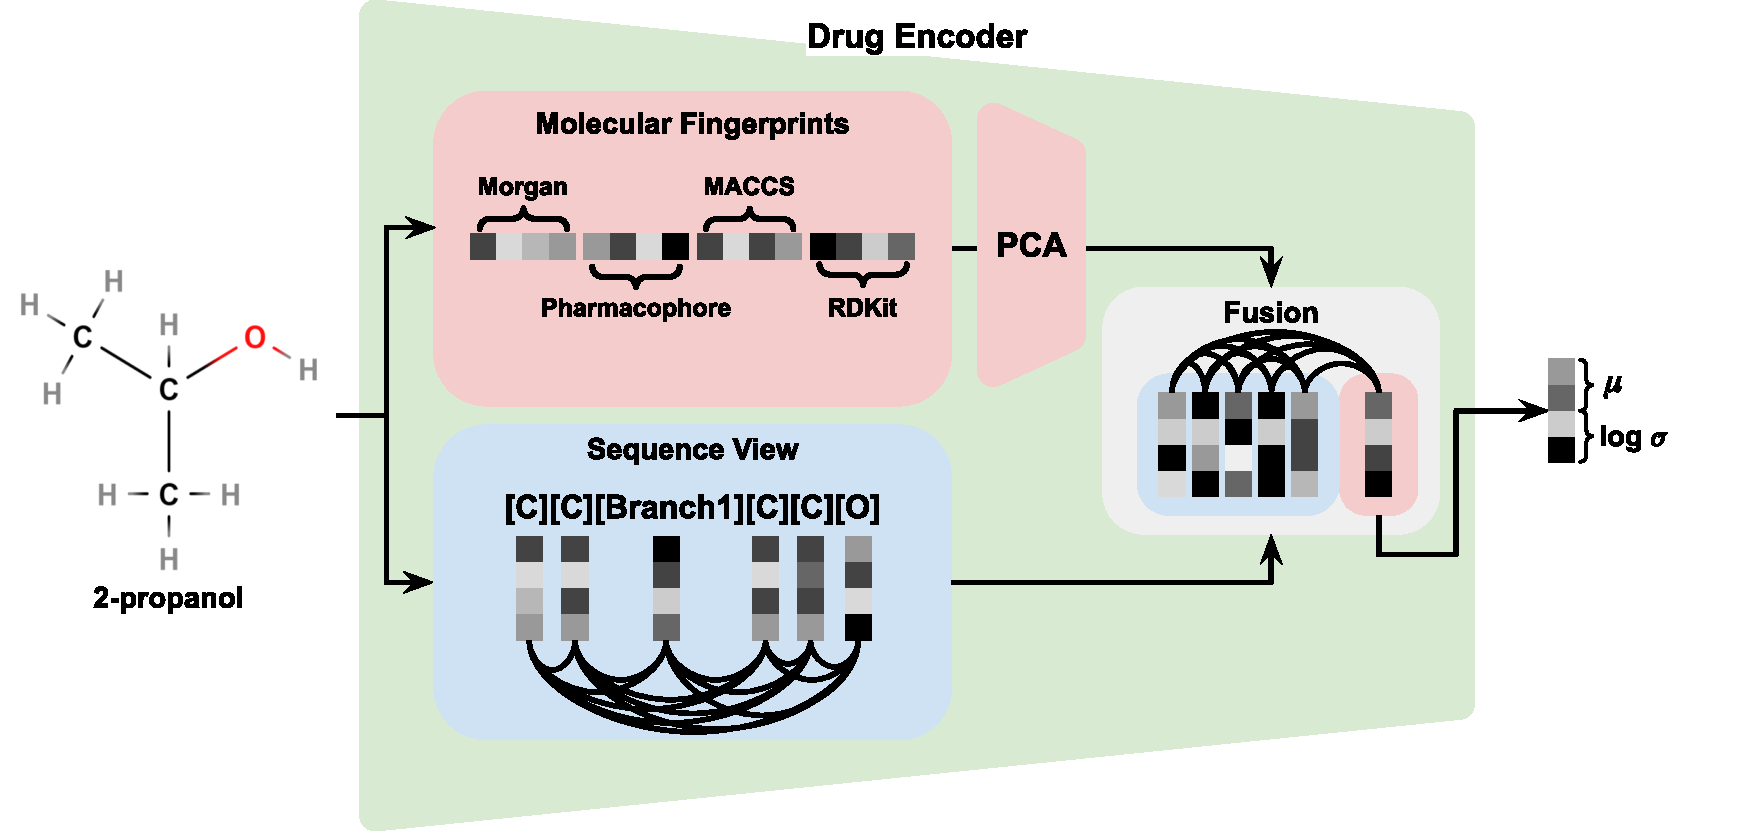
\includegraphics[width=\textwidth]{figs/model/drug_encoder.pdf}
    \end{figure}

    Fingerprints concatenated and projected to $\mathbb{R}^{256}$

    \vspace{0.2cm}

    SELFIES transformer in $\mathbb{R}^{L\times 256}$

    \vspace{0.2cm}

    The fusion block reads $\mu_d,\ \log\sigma_d \in \mathbb{R}^{128}$ off the
    fingerprint position

\end{frame}

\ours
\begin{frame}{SelVAEGen}
    \begin{figure}[h]
        \centering
        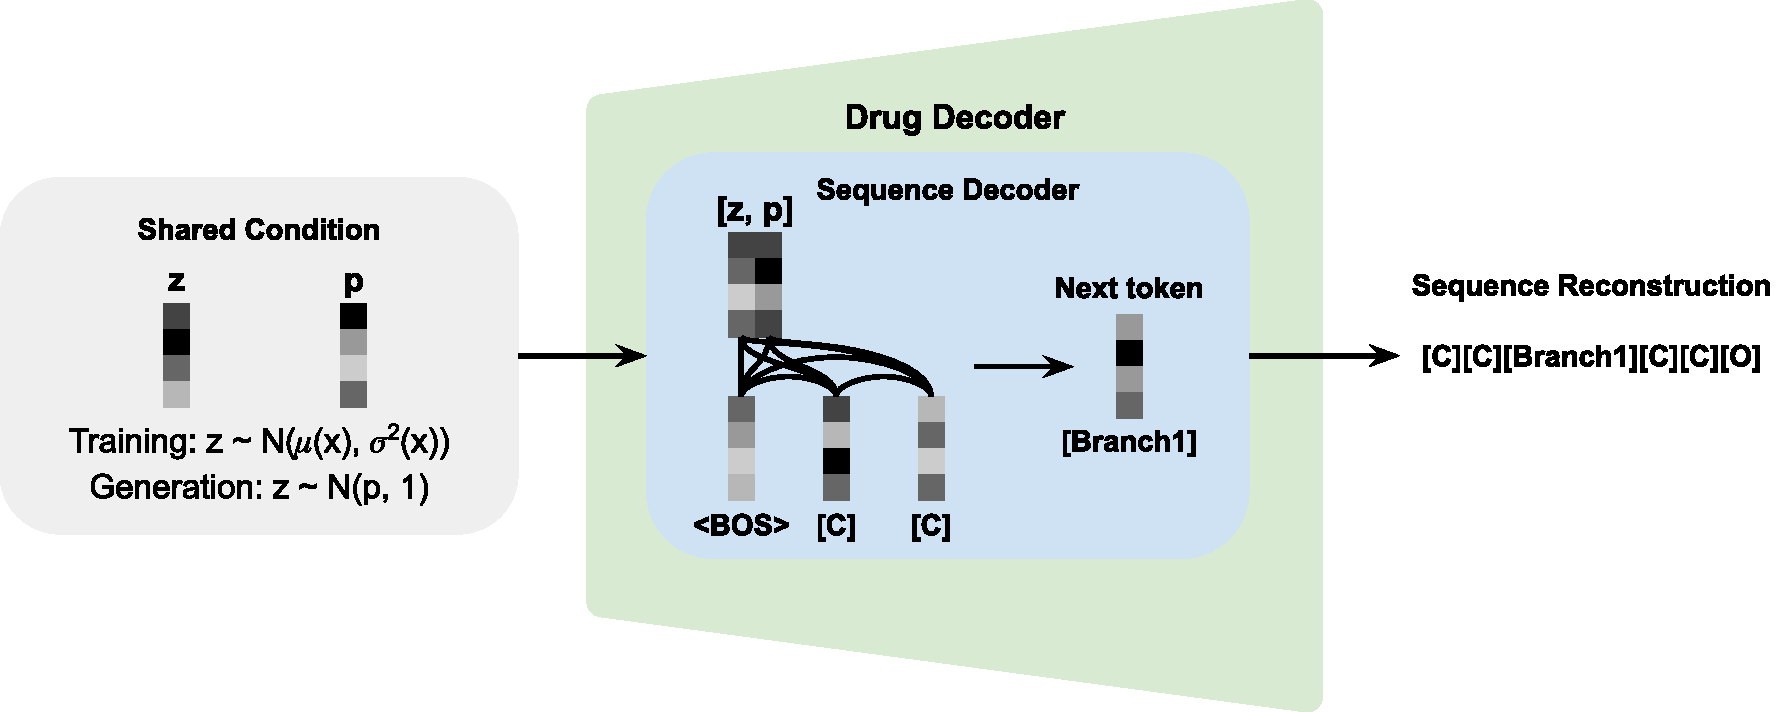
\includegraphics[width=\textwidth]{figs/model/drug_decoder.pdf}
    \end{figure}

    $z$ and $p$ are read by cross-attention

    \vspace{0.2cm}

    The decoder is a causal auto-regressive transformer in $\mathbb{R}^{L\times 256}$

    \vspace{0.2cm}

    One distribution over the SELFIES alphabet per position
\end{frame}

\ours
\begin{frame}[c]{New loss terms}
    \begin{center}
        Video time :)
    \end{center}
\end{frame}

\ours
\begin{frame}[c]{The full objective}
    We add our new losses to the VAE objective.

    \vspace{0.2cm}
    \[
    \begin{aligned}
        \mathcal{L} &={} \beta_{\mathrm{recon.}}\mathcal{L}_{\mathrm{recon.}}
        &&\text{reconstruct molecules}\\[0.7em]
        &+ \beta_{\mathrm{KL}}\,\mathcal{L}_\mathrm{KL}
        &&\text{regularization}\\[0.7em]
        &+ \beta_a\mathcal{L}_{\mathrm{aff}}
        &&\text{ranks two drugs relative to one protein}\\[0.7em]
        &+\beta_s\mathcal{L}_{\mathrm{sel}} &&\text{ranks two proteins relative to one drug}
    \end{aligned}
    \]
\end{frame}

\section{Results}

\begin{frame}[c]{The datasets}
    We test our model on 4 benchmark datasets.
    \bigskip

    Results are replicated 5 times with different data splits.

    \vfill

    \centering
    \renewcommand{\arraystretch}{1.8}
    \resizebox{\textwidth}{!}{%
        \begin{tabular}{lrrrrrr}
            \toprule
            \textbf{Dataset} & \textbf{Drugs} & \textbf{Proteins} & \textbf{Records} & \textbf{Density (\%)} & \textbf{Threshold} & \textbf{Positive (\%)} \\
            \midrule
            KIBA & 2,015 & 225 & 115,822 & 25.55 & 12.10 & 20.86 \\
            Davis & 64 & 427 & 27,328 & 100.00 & 7.00 & 8.03 \\
            BindingDB & 31,053 & 1,200 & 77,412 & 0.21 & 7.00 & 30.43 \\
            Papyrus & 81,147 & 749 & 239,226 & 0.39 & 7.00 & 32.15 \\
            \bottomrule
        \end{tabular}}

    \vfill
\end{frame}

\begin{frame}[c]{Our generated drugs are selective}
    \centering
    \makebox[\textwidth][c]{%
        
\includegraphics[width=1.16\textwidth]{figs/e6/kiba/seq_deltas.pdf}%
    }

    \makebox[\textwidth][c]{%
        
\includegraphics[width=1.16\textwidth]{figs/e6/kiba/seq_agreement.pdf}%
    }
\end{frame}

\begin{frame}[c]{And the affinity is higher too}
    \centering
    \makebox[\textwidth][c]{%
        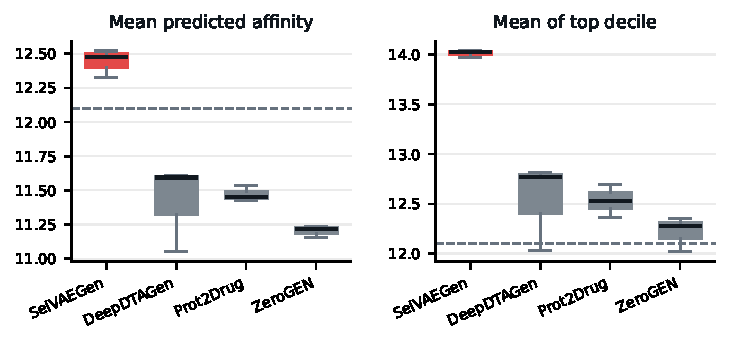
\includegraphics[width=1.10\textwidth]{figs/talk/quality_affinity.pdf}%
    }
\end{frame}

\begin{frame}[c]{This is not at the cost of chemical quality}
    \centering
    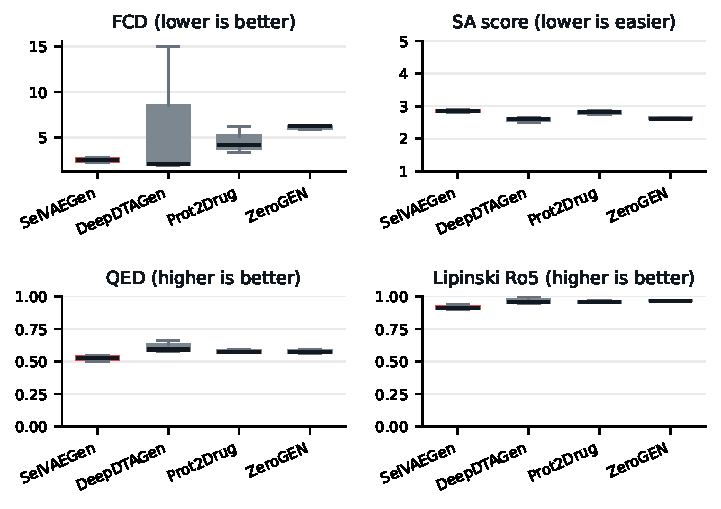
\includegraphics[width=\textwidth,height=0.88\textheight,keepaspectratio]
    {figs/talk/quality_chemistry.pdf}
\end{frame}

\begin{frame}[c]{We generate drugs with higher affinity}
    \centering
    \makebox[\textwidth][c]{%
        
\includegraphics[width=1.10\textwidth]{figs/e7/kiba/affinity.pdf}%
    }
\end{frame}

\begin{frame}[c]{Difference in $p_G$ and $q_G$}
    In KIBA:

    \vfill

    \centering
    \makebox[\textwidth][c]{%
        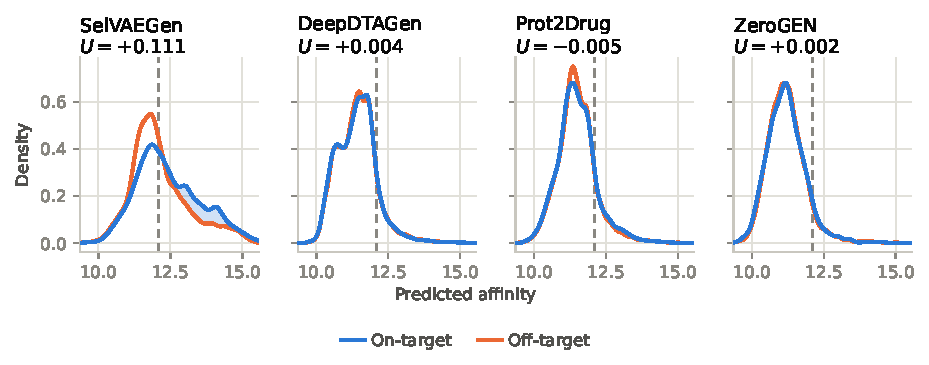
\includegraphics[width=1.16\textwidth]{figs/talk/side_by_side_kiba.pdf}%
    }

    \vfill
\end{frame}

\begin{frame}[c]{Difference in $p_G$ and $q_G$}
    \centering
    \makebox[\textwidth][c]{%
        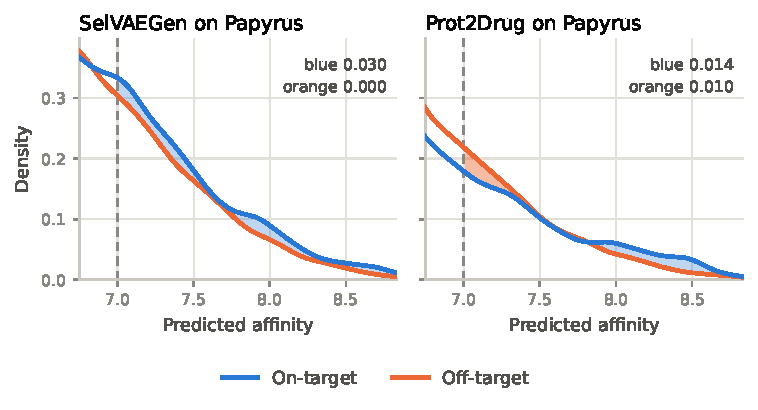
\includegraphics[width=1.16\textwidth]{figs/talk/tail_zoom.pdf}%
    }
\end{frame}

\begin{frame}[t]{Utility}
    \begin{table}
        \centering

        \small
        \begin{tabular}{clc}
            \toprule
            Dataset & Model
            & Utility \\
            \midrule

            \multirow{4}{*}{KIBA} & SelVAEGen
            & \textbf{0.1334 $\pm$ 0.0499} \\
            & DeepDTAGen
            & \textbf{0.0045 $\pm$ 0.0016} \\
            & Prot2Drug
            & \textbf{0.0165 $\pm$ 0.0017} \\
            & ZeroGEN
            & \textbf{0.0046 $\pm$ 0.0024} \\
            \midrule

            \multirow{4}{*}{Davis} & SelVAEGen
            & \textbf{0.2013 $\pm$ 0.0375} \\
            & DeepDTAGen
            & -0.0002 $\pm$ 0.0004 \\
            & Prot2Drug
            & 0.0001 $\pm$ 0.0015 \\
            & ZeroGEN
            & 0.0012 $\pm$ 0.0011 \\
            \midrule

            \multirow{4}{*}{BindingDB} & SelVAEGen
            & \textbf{0.0275 $\pm$ 0.0050} \\
            & DeepDTAGen
            & \textbf{0.0060 $\pm$ 0.0026} \\
            & Prot2Drug
            & -0.0001 $\pm$ 0.0086 \\
            & ZeroGEN
            & 0.0063 $\pm$ 0.0116 \\
            \midrule

            \multirow{4}{*}{Papyrus} & SelVAEGen
            & \textbf{0.0373 $\pm$ 0.0222} \\
            & DeepDTAGen
            & -0.0023 $\pm$ 0.0019 \\
            & Prot2Drug
            & 0.0040 $\pm$ 0.0132 \\
            & ZeroGEN
            & -0.0004 $\pm$ 0.0057 \\

            \bottomrule
        \end{tabular}
    \end{table}
\end{frame}

\begin{frame}[t]{Sparsity, not size}
    \centering
    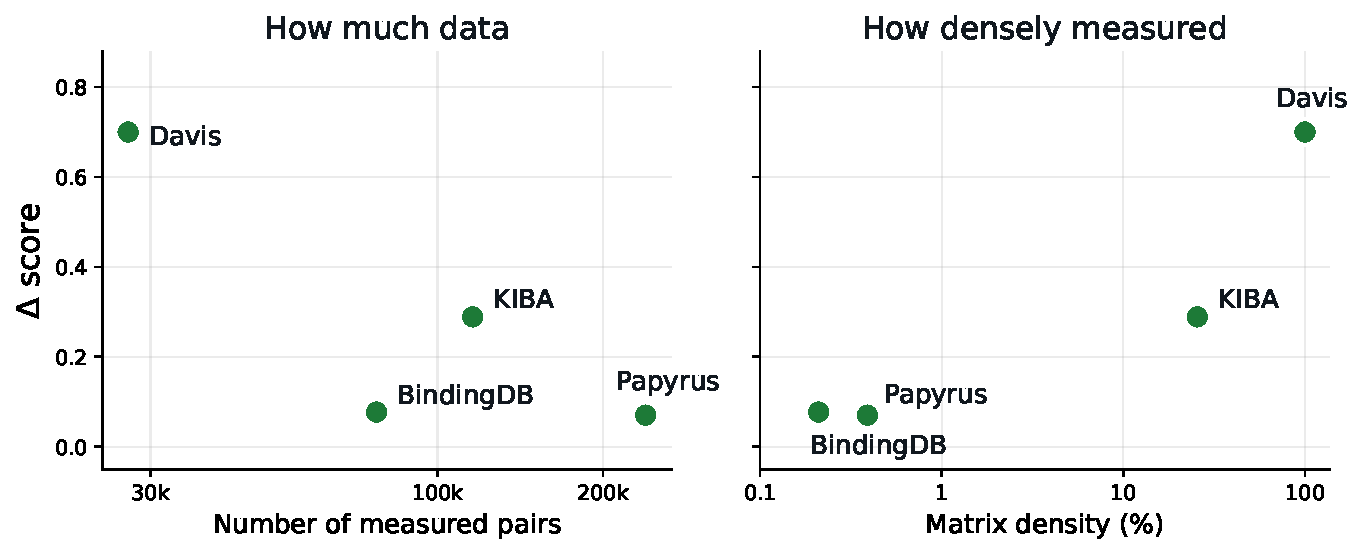
\includegraphics[width=\textwidth]{figs/talk/density_not_size.pdf}

    \vfill
    \raggedright
    Davis is the \textbf{smallest} dataset and the \textbf{most dense}.

    Papyrus is the \textbf{largest} dataset but the second \textbf{most sparse}.

    \vspace{0.3cm}

    \textcolor{red}{$\mathcal{L}_{\mathrm{sel}}$ needs the same drug measured against two
        proteins.}
\end{frame}

\section{Conclusion}
\begin{frame}{Conclusion}
    \begin{itemize}
        \item We uniformize a notion that is spread throughout the literature
        \item We formalize it into a well-defined ML task
        \item We define additional metrics to identify selectivity
        \item We show that current models' generation is not selective
        \item We derive loss functions that promote it
        \item We introduce a model capable of selective drug generation
    \end{itemize}
\end{frame}

\begin{frame}{Limitations and future work}
    \begin{itemize}
        \item \textbf{Predicted (not measured) selectivity.}

        So far, we rely on oracle predictions.

        \medskip
        $\Longrightarrow$ Validate with docking experiments.

        \vfill

        \medskip
        \item \textbf{Whole-protein conditioning.}

        We currently condition on the entire protein sequence.

        \medskip
        $\Longrightarrow$ Extend to specific binding pockets or interfaces.
    \end{itemize}
\end{frame}

\section*{Thanks}
\begin{frame}[plain, c]
    \begin{center}
        \Huge
        Thank you!

        \vspace{1cm}

        \normalsize
        Questions?
    \end{center}
\end{frame}

\pdfstringdefDisableCommands{\renewcommand{\translate}[1]{#1}}
\appendix

\newcounter{framenumberbeforebackup}
\setcounter{framenumberbeforebackup}{\value{framenumber}}

\newsavebox{\backupcaption}
\newcommand{\backupfigure}[2]{%
    \sbox{\backupcaption}{\parbox{\textwidth}{\raggedright\scriptsize #1}}%
    \centering
    \includegraphics[width=\textwidth,
        height=\dimexpr\textheight-\ht\backupcaption-\dp\backupcaption-1.9em\relax,
        keepaspectratio]{#2}%
    \par\vspace{0.5em}%
    \usebox{\backupcaption}%
}
\newcommand{\backuptable}[2]{%
    \sbox{\backupcaption}{\parbox{\textwidth}{\raggedright\scriptsize #1}}%
    \centering
    \resizebox{\textwidth}{!}{#2}%
    \par\vspace{0.5em}%
    \usebox{\backupcaption}%
}

\begin{frame}[plain]
    \backupfigure{\textbf{Figure 1.} Binding between a protein (gray structure) and a drug (colored structure). The drug binds to the protein structure and disrupts its biological function.}{figs/chapters/1.pdf}
\end{frame}

\begin{frame}[plain]
    \backupfigure{\textbf{Figure 2.} Progression of research questions in the field of drug generation. At first, models were concerned with generating drugs with a similar distribution to the training set. Then, a series of models were developed in order to integrate protein target information to guide generation. Nowadays, an increasing number of models attempt to generate drugs optimizing for on-target affinity. At the same time, preliminary concerns have been raised regarding the selectivity of generated drugs. This work proposes to formalize this concern, define rigorous metrics to diagnose it and improve selectivity via new training objectives.}{figs/chapters/2.pdf}
\end{frame}

\begin{frame}[plain]
    \backupfigure{\textbf{Figure 3.} The variational autoencoder. An encoder maps an observation to a probability distribution over latent representations. A sample is taken from that distribution, and a decoder reconstructs the observation from it. Training balances reconstruction and a divergence term that keeps the encoder's distribution close to a prior. By learning to map data to a distribution close to this prior, the model later is able to sample from the prior and decode new data. Source:.}{figs/model/VAE.pdf}
\end{frame}

\begin{frame}[plain]
    \backupfigure{\textbf{Figure 4.} Three molecules shown as structures together with the two string notations that denote them. SMILES encodes branches with parentheses and rings with paired digits, so the digit opening a ring is a commitment the remainder of the string must honor and a syntactically plausible string can still denote no molecule at all. SELFIES replaces this with bracketed tokens whose meaning is resolved against the valences still available as the string is read, so every sequence of tokens decodes to a valid structure. Both notations follow the usual convention of leaving hydrogens implicit. Those are recovered when the string is read.}{figs/model/notations.pdf}
\end{frame}

\begin{frame}[plain]
    \backupfigure{\textbf{Figure 5.} Geometric interpretation of utility. In its most general sense, a generator is selective if the drugs it generates have higher affinity values for the proteins they were designed for than for other proteins. $p_G$ is the distribution of on-target affinities, and $q_G$ is the distribution of off-target affinities. If we measure the difference in the areas of each curve above a biologically relevant threshold $\tau$, we get a value called utility. We show in Proposition 3.1 that integrating this utility over all possible $\tau$ values yields the $\Delta$ score discussed previously.}{figs/chapters/metrics.pdf}
\end{frame}

\begin{frame}[plain]
    \backupfigure{\textbf{Figure 6.} Variational drug encoding. A molecule is represented by a Gaussian distribution whose mean and variance are obtained from its chemical structure. Each protein defines another Gaussian in the same latent space, with a learned mean and fixed variance. Training places molecules closer to proteins for which their measured affinity is higher and further from those for which it is lower. Generation then samples from the region associated with the requested protein and decodes the sample into a molecule.}{figs/chapters/methods.pdf}
\end{frame}

\begin{frame}[plain]
    \backupfigure{\textbf{Figure 7.} The complete SelVAEGen architecture. During training, the drug encoder supplies a posterior sample $z$ (dashed arrow) and the decoder reconstructs the input molecule. During generation, the drug encoder is unused and $z$ is sampled from the protein-conditioned prior (dotted arrow). The decoder receives the latent sample and protein representation in both cases.}{figs/model/model.pdf}
\end{frame}

\begin{frame}[plain]
    \backupfigure{\textbf{Figure 8.} The protein encoder. A frozen ESM-C model produces residue embeddings, which are averaged, standardized, and reduced by PCA to the fixed representation $e(P)$. A residual adapter maps this representation to the protein prior mean $m_\psi(P)$.}{figs/model/protein_encoder.pdf}
\end{frame}

\begin{frame}[plain]
    \backupfigure{\textbf{Figure 9.} The drug encoder. Fixed molecular fingerprints and token-level SELFIES representations are combined by a fusion Transformer. The state at the fingerprint position is projected into the parameters $\mu_d$ and $\log\sigma_d^2$ of the molecular posterior.}{figs/model/drug_encoder.pdf}
\end{frame}

\begin{frame}[plain]
    \backupfigure{\textbf{Figure 10.} The autoregressive drug decoder. The latent representation and protein representation are supplied through cross-attention, while protein-dependent affine transformations provide additional conditioning after each Transformer layer.}{figs/model/drug_decoder.pdf}
\end{frame}

\begin{frame}[plain]
    \backupfigure{\textbf{Figure 11.} How the losses organize the latent space. \textbf{(a)} The reconstruction loss requires the code to retain molecular information from which the decoder can recover the input string. \textbf{(b)} The prior regularization loss brings the molecular posterior mean $\mu_d$ towards the conditioning protein's Gaussian and its variance towards one, matching the distribution used for generation. \textbf{(c)} The affinity ranking loss compares two molecules for one protein and encourages the stronger measured binder to have higher compatibility by the margin $\eta_{\mathrm{aff}}$. \textbf{(d)} The selectivity ranking loss compares one molecule against two proteins and encourages higher compatibility with the protein it binds more strongly. In both ranking panels the dimension lines mark the latent spans that the compatibility score reads.}{figs/model/losses.pdf}
\end{frame}

\begin{frame}[plain]
    \backupfigure{\textbf{Figure 12.} Predicted on-target and ranked off-target affinities on KIBA. For each of the 23 test proteins, each model generates 256 molecules. Colored bars show the mean predicted affinity to the conditioning protein. Gray bars show the mean predicted affinity to off-target proteins after ranking them by affinity, so that the first gray bar corresponds to the strongest predicted off-target, the second to the second strongest, and so on. The dashed line indicates the dataset’s positive-affinity threshold. The $\Delta$ score is defined as the height of the colored bar minus the mean height of the gray bars. Among the models compared, SelVAEGen is the only one that shows both a positive $\Delta$ score and a mean on-target affinity above the dataset’s threshold.}{figs/chapters/results.pdf}
\end{frame}

\begin{frame}[plain]
    \backupfigure{\textbf{Figure 13.} Profile of the KIBA dataset. \textbf{(a)} Distribution of recorded affinity values, with the dataset's positive-affinity threshold marked in red. \textbf{(b)} Distribution of protein lengths, measured as the number of amino acids in each unique protein. \textbf{(c)} Distribution of molecular string lengths for unique drugs. The red lines in \textbf{(b)} and \textbf{(c)} mark the filtering criteria. \textbf{(d)} Number of recorded affinity measurements per protein.}{figs/e0/kiba/distributions.pdf}
\end{frame}

\begin{frame}[plain]
    \backupfigure{\textbf{Figure 14.} Profile of the Davis dataset. \textbf{(a)} Distribution of recorded affinity values, with the dataset's positive-affinity threshold marked in red. \textbf{(b)} Distribution of protein lengths, measured as the number of amino acids in each unique protein. \textbf{(c)} Distribution of molecular string lengths for unique drugs. The red lines in \textbf{(b)} and \textbf{(c)} mark the filtering criteria. \textbf{(d)} Number of recorded affinity measurements per protein.}{figs/e0/davis/distributions.pdf}
\end{frame}

\begin{frame}[plain]
    \backupfigure{\textbf{Figure 15.} Profile of the BindingDB dataset. \textbf{(a)} Distribution of recorded affinity values, with the dataset's positive-affinity threshold marked in red. \textbf{(b)} Distribution of protein lengths, measured as the number of amino acids in each unique protein. \textbf{(c)} Distribution of molecular string lengths for unique drugs. The red lines in \textbf{(b)} and \textbf{(c)} mark the filtering criteria. \textbf{(d)} Number of recorded affinity measurements per protein.}{figs/e0/bindingdb/distributions.pdf}
\end{frame}

\begin{frame}[plain]
    \backupfigure{\textbf{Figure 16.} Profile of the Papyrus dataset. \textbf{(a)} Distribution of recorded affinity values, with the dataset's positive-affinity threshold marked in red. \textbf{(b)} Distribution of protein lengths, measured as the number of amino acids in each unique protein. \textbf{(c)} Distribution of molecular string lengths for unique drugs. The red lines in \textbf{(b)} and \textbf{(c)} mark the filtering criteria. \textbf{(d)} Number of recorded affinity measurements per protein.}{figs/e0/papyrus/distributions.pdf}
\end{frame}

\begin{frame}[plain]
    \backuptable{\textbf{Table 1.} Dataset statistics after the curation criteria above have been applied. \textbf{Drugs} and \textbf{Proteins} count the distinct molecules and distinct proteins that survive filtering. \textbf{Records} is the number of observed drug-protein affinities. \textbf{Density} expresses those records as a percentage of the $\text{Drugs}\times\text{Proteins}$ pairs that could in principle have been measured, so $100\%$ means every drug was tested against every protein and a small value means most of the matrix is unobserved. \textbf{Threshold} is the value on that dataset's own affinity scale at or above which a pair is treated as binding, which differs because KIBA reports a composite KIBA score while the other three report affinities on the $pKd$ scale. \textbf{Positive} is the percentage of records reaching that threshold.}{%
        \begin{tabular}{lrrrrrr}
            \toprule
            \textbf{Dataset} & \textbf{Drugs} & \textbf{Proteins} & \textbf{Records} & \textbf{Density (\%)} & \textbf{Threshold}& \textbf{Positive (\%)} \\
            \midrule
            KIBA & 2,015 & 225 & 115,822 & 25.55 & 12.10 & 20.86 \\
            Davis & 64 & 427 & 27,328 & 100.00 & 7.00 & 8.03 \\
            BindingDB & 31,053 & 1,200 & 77,412 & 0.21 & 7.00 & 30.43 \\
            Papyrus & 81,147 & 749 & 239,226 & 0.39 & 7.00 & 32.15 \\
            \bottomrule
        \end{tabular}
    }
\end{frame}

\begin{frame}[plain]
    \backupfigure{\textbf{Figure 17 (1 of 4, KIBA).} The twenty drugs with the highest empirical $\Delta$ score among those measured against at least three proteins in \textbf{(a)} KIBA, \textbf{(b)} Davis, \textbf{(c)} BindingDB and \textbf{(d)} Papyrus. Each row is one drug, and the columns are the proteins preferred by these drugs, arranged so that each diagonal entry is the drug's best measured target. Cell color represents measured affinity. Blank cells indicate unmeasured pairs. Grayscale cells indicate affinity values below the dataset's threshold, and cells in green scale indicate higher affinity values. The strip on the right follows the same row order and gives each drug's empirical $\Delta$: its affinity for the best target minus its mean measured affinity for the remaining proteins, with a bootstrap interval over the off-target set. These examples use experimental data directly, without an oracle or generator.}{figs/e0/kiba/selectivity.pdf}
\end{frame}

\begin{frame}[plain]
    \backupfigure{\textbf{Figure 17 (2 of 4, Davis).} The twenty drugs with the highest empirical $\Delta$ score among those measured against at least three proteins in \textbf{(a)} KIBA, \textbf{(b)} Davis, \textbf{(c)} BindingDB and \textbf{(d)} Papyrus. Each row is one drug, and the columns are the proteins preferred by these drugs, arranged so that each diagonal entry is the drug's best measured target. Cell color represents measured affinity. Blank cells indicate unmeasured pairs. Grayscale cells indicate affinity values below the dataset's threshold, and cells in green scale indicate higher affinity values. The strip on the right follows the same row order and gives each drug's empirical $\Delta$: its affinity for the best target minus its mean measured affinity for the remaining proteins, with a bootstrap interval over the off-target set. These examples use experimental data directly, without an oracle or generator.}{figs/e0/davis/selectivity.pdf}
\end{frame}

\begin{frame}[plain]
    \backupfigure{\textbf{Figure 17 (3 of 4, BindingDB).} The twenty drugs with the highest empirical $\Delta$ score among those measured against at least three proteins in \textbf{(a)} KIBA, \textbf{(b)} Davis, \textbf{(c)} BindingDB and \textbf{(d)} Papyrus. Each row is one drug, and the columns are the proteins preferred by these drugs, arranged so that each diagonal entry is the drug's best measured target. Cell color represents measured affinity. Blank cells indicate unmeasured pairs. Grayscale cells indicate affinity values below the dataset's threshold, and cells in green scale indicate higher affinity values. The strip on the right follows the same row order and gives each drug's empirical $\Delta$: its affinity for the best target minus its mean measured affinity for the remaining proteins, with a bootstrap interval over the off-target set. These examples use experimental data directly, without an oracle or generator.}{figs/e0/bindingdb/selectivity.pdf}
\end{frame}

\begin{frame}[plain]
    \backupfigure{\textbf{Figure 17 (4 of 4, Papyrus).} The twenty drugs with the highest empirical $\Delta$ score among those measured against at least three proteins in \textbf{(a)} KIBA, \textbf{(b)} Davis, \textbf{(c)} BindingDB and \textbf{(d)} Papyrus. Each row is one drug, and the columns are the proteins preferred by these drugs, arranged so that each diagonal entry is the drug's best measured target. Cell color represents measured affinity. Blank cells indicate unmeasured pairs. Grayscale cells indicate affinity values below the dataset's threshold, and cells in green scale indicate higher affinity values. The strip on the right follows the same row order and gives each drug's empirical $\Delta$: its affinity for the best target minus its mean measured affinity for the remaining proteins, with a bootstrap interval over the off-target set. These examples use experimental data directly, without an oracle or generator.}{figs/e0/papyrus/selectivity.pdf}
\end{frame}

\begin{frame}[plain]
    \backuptable{\textbf{Table 2.} How much selectivity information each dataset holds. A comparison is a pair of proteins measured against one common drug, which is the unit the selectivity ranking loss of Section 4.3 consumes. A drug measured against $n$ proteins supplies $\binom{n}{2}$ of them, and a drug measured against one supplies none. \textbf{Drugs} is the number of distinct molecules. \textbf{Per drug} is the mean number of affinity records per drug. \textbf{$\geq 2$ targets} is the percentage of drugs measured against at least two distinct proteins, which is the percentage contributing any comparison at all. The remainder of each dataset contributes none. \textbf{Comparisons} is $\sum_d \binom{n_d}{2}$ over every drug $d$, the total the dataset supplies, and \textbf{Top 1\%} is the share of that total coming from the $1\%$ of drugs measured against the most proteins.}{%
        \begin{tabular}{lrrrrr}
            \toprule
            \textbf{Dataset} & \textbf{Drugs} & \textbf{Per drug} &
            \textbf{$\geq 2$ targets} & \textbf{Comparisons} & \textbf{Top 1\%} \\
            \midrule
            KIBA      &  2,015 &  57.5 & 100.0\% & 5,653,431 &  4.3\% \\
            Davis     &     64 & 427.0 & 100.0\% & 5,820,864 &  1.6\% \\
            BindingDB & 31,053 &   2.5 &  23.9\% & 5,617,163 & 99.6\% \\
            Papyrus   & 81,147 &   2.9 &  40.5\% & 5,422,313 & 93.7\% \\
            \bottomrule
        \end{tabular}
    }
\end{frame}

\begin{frame}[plain]
    \backupfigure{\textbf{Figure 18.} Recorded affinities grouped by drug in the left column and by protein in the right. Rows correspond to \textbf{(a, b)} KIBA, \textbf{(c, d)} Davis, \textbf{(e, f)} BindingDB and \textbf{(g, h)} Papyrus. Each purple square is one measurement, the blue line is the group mean, and the red dashed line is the dataset's positive-affinity threshold. Groups are ordered horizontally by mean affinity. The two panels in each row share a vertical scale. The left column shows the measurements available for comparing proteins for a fixed drug, as required by the selectivity ranking loss. The two largest datasets concentrate more measurements per protein than per drug.}{figs/e0/affinity_full.pdf}
\end{frame}

\begin{frame}[plain]
    \backupfigure{\textbf{Figure 19.} The affinity groups of Figure 18, reduced to fifty evenly spaced drugs in the left column and fifty evenly spaced proteins in the right. Rows correspond to \textbf{(a, b)} KIBA, \textbf{(c, d)} Davis, \textbf{(e, f)} BindingDB and \textbf{(g, h)} Papyrus. Groups are selected at a fixed stride through the ordering by mean affinity. Each purple square is one measurement: dense columns indicate groups with many observations, while columns with two or three squares indicate limited coverage. For the drug groups on the left, this coverage determines how many protein preferences can be compared. Davis retains its complete drug panel because it contains only $64$ drugs. BindingDB's and Papyrus's sparsity is evident in the thin columns.}{figs/e0/affinity_thinned.pdf}
\end{frame}

\begin{frame}[plain]
    \backuptable{\textbf{Table 3.} Oracle performance on each dataset's test set of measured drug-protein pairs. RMSE measures prediction error, CI measures agreement with observed affinity rankings, and Directional Consistency measures how often the oracle correctly orders the affinities of two proteins for a fixed drug. Lower RMSE and higher values of the two ranking metrics are desirable.}{%
        \begin{tabular}{llccc}
            \toprule
            \textbf{Dataset} & \textbf{Oracle} & \textbf{RMSE} & \textbf{CI} & \textbf{Dir. consistency} \\
            \midrule
            KIBA & Baseline & 0.4544 & 0.8193 & 0.7658 \\
            KIBA & GraphDTA & 0.5080 & 0.8169 & 0.7514 \\
            KIBA & GSDTA & 0.4478 & 0.8432 & 0.7927 \\
            \midrule
            Davis & Baseline & 0.5150 & 0.8672 & 0.8322 \\
            Davis & GraphDTA & 0.5556 & 0.8645 & 0.7947 \\
            Davis & GSDTA & 0.5520 & 0.8612 & 0.7972 \\
            \midrule
            BindingDB & Baseline & 0.7585 & 0.8692 & 0.7639 \\
            BindingDB & GraphDTA & 0.7613 & 0.8675 & 0.7557 \\
            BindingDB & GSDTA & 0.7448 & 0.8756 & 0.7686 \\
            \midrule
            Papyrus & Baseline & 0.6532 & 0.8374 & 0.7439 \\
            Papyrus & GraphDTA & 0.6361 & 0.8493 & 0.7829 \\
            Papyrus & GSDTA & 0.5925 & 0.8646 & 0.8280 \\
            \bottomrule
        \end{tabular}
    }
\end{frame}

\begin{frame}[plain]
    \backupfigure{\textbf{Figure 20 (1 of 3, Baseline oracle).} QQ-plots comparing predicted and observed affinity values on KIBA for \textbf{(a)} the baseline oracle, \textbf{(b)} GraphDTA and \textbf{(c)} GSDTA. Corresponding quantiles show how the predicted affinity distribution relates to the observed one across its range, including the low- and high-affinity extremes.}{figs/oracles/kiba/BaselineOracle_qq_predicted.pdf}
\end{frame}

\begin{frame}[plain]
    \backupfigure{\textbf{Figure 20 (2 of 3, GraphDTA).} QQ-plots comparing predicted and observed affinity values on KIBA for \textbf{(a)} the baseline oracle, \textbf{(b)} GraphDTA and \textbf{(c)} GSDTA. Corresponding quantiles show how the predicted affinity distribution relates to the observed one across its range, including the low- and high-affinity extremes.}{figs/oracles/kiba/GraphDTAOracle_qq_predicted.pdf}
\end{frame}

\begin{frame}[plain]
    \backupfigure{\textbf{Figure 20 (3 of 3, GSDTA).} QQ-plots comparing predicted and observed affinity values on KIBA for \textbf{(a)} the baseline oracle, \textbf{(b)} GraphDTA and \textbf{(c)} GSDTA. Corresponding quantiles show how the predicted affinity distribution relates to the observed one across its range, including the low- and high-affinity extremes.}{figs/oracles/kiba/GSDTAOracle_qq_predicted.pdf}
\end{frame}

\begin{frame}[plain]
    \backupfigure{\textbf{Figure 21 (1 of 4, KIBA).} Oracle disagreement in \textbf{(a)} KIBA, \textbf{(b)} Davis, \textbf{(c)} BindingDB and \textbf{(d)} Papyrus. Disagreement is the standard deviation of the three oracle predictions for one drug-protein pair. The left panel compares the disagreement recorded on generated molecules with that recorded on training molecules. The middle panel asks whether disagreement tracks how unfamiliar a molecule is, measuring familiarity as the Tanimoto similarity of a generated molecule to the nearest molecule in the training set. The right panel asks whether disagreement tracks error. In both of the right-hand panels the generated molecules or measured pairs are sorted by disagreement and split into ten bins of equal count: each marker is one bin, at the mean disagreement of its members and the mean Tanimoto similarity or root mean squared error within it.}{figs/e7/kiba/oracle_disagreement_panels.pdf}
\end{frame}

\begin{frame}[plain]
    \backupfigure{\textbf{Figure 21 (2 of 4, Davis).} Oracle disagreement in \textbf{(a)} KIBA, \textbf{(b)} Davis, \textbf{(c)} BindingDB and \textbf{(d)} Papyrus. Disagreement is the standard deviation of the three oracle predictions for one drug-protein pair. The left panel compares the disagreement recorded on generated molecules with that recorded on training molecules. The middle panel asks whether disagreement tracks how unfamiliar a molecule is, measuring familiarity as the Tanimoto similarity of a generated molecule to the nearest molecule in the training set. The right panel asks whether disagreement tracks error. In both of the right-hand panels the generated molecules or measured pairs are sorted by disagreement and split into ten bins of equal count: each marker is one bin, at the mean disagreement of its members and the mean Tanimoto similarity or root mean squared error within it.}{figs/e7/davis/oracle_disagreement_panels.pdf}
\end{frame}

\begin{frame}[plain]
    \backupfigure{\textbf{Figure 21 (3 of 4, BindingDB).} Oracle disagreement in \textbf{(a)} KIBA, \textbf{(b)} Davis, \textbf{(c)} BindingDB and \textbf{(d)} Papyrus. Disagreement is the standard deviation of the three oracle predictions for one drug-protein pair. The left panel compares the disagreement recorded on generated molecules with that recorded on training molecules. The middle panel asks whether disagreement tracks how unfamiliar a molecule is, measuring familiarity as the Tanimoto similarity of a generated molecule to the nearest molecule in the training set. The right panel asks whether disagreement tracks error. In both of the right-hand panels the generated molecules or measured pairs are sorted by disagreement and split into ten bins of equal count: each marker is one bin, at the mean disagreement of its members and the mean Tanimoto similarity or root mean squared error within it.}{figs/e7/bindingdb/oracle_disagreement_panels.pdf}
\end{frame}

\begin{frame}[plain]
    \backupfigure{\textbf{Figure 21 (4 of 4, Papyrus).} Oracle disagreement in \textbf{(a)} KIBA, \textbf{(b)} Davis, \textbf{(c)} BindingDB and \textbf{(d)} Papyrus. Disagreement is the standard deviation of the three oracle predictions for one drug-protein pair. The left panel compares the disagreement recorded on generated molecules with that recorded on training molecules. The middle panel asks whether disagreement tracks how unfamiliar a molecule is, measuring familiarity as the Tanimoto similarity of a generated molecule to the nearest molecule in the training set. The right panel asks whether disagreement tracks error. In both of the right-hand panels the generated molecules or measured pairs are sorted by disagreement and split into ten bins of equal count: each marker is one bin, at the mean disagreement of its members and the mean Tanimoto similarity or root mean squared error within it.}{figs/e7/papyrus/oracle_disagreement_panels.pdf}
\end{frame}

\begin{frame}[plain]
    \backupfigure{\textbf{Figure 22 (1 of 4, KIBA).} Validity, uniqueness and novelty of generated molecules in \textbf{(a)} KIBA, \textbf{(b)} Davis, \textbf{(c)} BindingDB and \textbf{(d)} Papyrus. Each row corresponds to results of the dataset mentioned in the left. Validity measures how often a generation attempt produces a parsable molecule, uniqueness measures how much of the valid output is distinct, and novelty measures how much is absent from the training set. All four models were trained from scratch on the same splits with the same tokenizer.}{figs/e6/kiba/seq_quality.pdf}
\end{frame}

\begin{frame}[plain]
    \backupfigure{\textbf{Figure 22 (2 of 4, Davis).} Validity, uniqueness and novelty of generated molecules in \textbf{(a)} KIBA, \textbf{(b)} Davis, \textbf{(c)} BindingDB and \textbf{(d)} Papyrus. Each row corresponds to results of the dataset mentioned in the left. Validity measures how often a generation attempt produces a parsable molecule, uniqueness measures how much of the valid output is distinct, and novelty measures how much is absent from the training set. All four models were trained from scratch on the same splits with the same tokenizer.}{figs/e6/davis/seq_quality.pdf}
\end{frame}

\begin{frame}[plain]
    \backupfigure{\textbf{Figure 22 (3 of 4, BindingDB).} Validity, uniqueness and novelty of generated molecules in \textbf{(a)} KIBA, \textbf{(b)} Davis, \textbf{(c)} BindingDB and \textbf{(d)} Papyrus. Each row corresponds to results of the dataset mentioned in the left. Validity measures how often a generation attempt produces a parsable molecule, uniqueness measures how much of the valid output is distinct, and novelty measures how much is absent from the training set. All four models were trained from scratch on the same splits with the same tokenizer.}{figs/e6/bindingdb/seq_quality.pdf}
\end{frame}

\begin{frame}[plain]
    \backupfigure{\textbf{Figure 22 (4 of 4, Papyrus).} Validity, uniqueness and novelty of generated molecules in \textbf{(a)} KIBA, \textbf{(b)} Davis, \textbf{(c)} BindingDB and \textbf{(d)} Papyrus. Each row corresponds to results of the dataset mentioned in the left. Validity measures how often a generation attempt produces a parsable molecule, uniqueness measures how much of the valid output is distinct, and novelty measures how much is absent from the training set. All four models were trained from scratch on the same splits with the same tokenizer.}{figs/e6/papyrus/seq_quality.pdf}
\end{frame}

\begin{frame}[plain]
    \backupfigure{\textbf{Figure 23 (1 of 4, KIBA).} Predicted potency and distributional similarity of generated molecules in \textbf{(a)} KIBA, \textbf{(b)} Davis, \textbf{(c)} BindingDB and \textbf{(d)} Papyrus. Mean predicted affinity summarizes the whole library, while the mean of the top decile summarizes its best tenth, the candidates of greatest interest for subsequent selection. Success rate counts unique, novel molecules whose predicted affinity clears the dataset threshold, marked by a dashed line in the first two panels. Fr\'echet ChemNet distance compares the generated and training chemical distributions; lower values indicate a closer match, making this the only panel where lower is better. BindingDB and Papyrus provide roughly three measurements per drug, so their affinity estimates draw on sparser data than KIBA and Davis.}{figs/e6/kiba/seq_potency.pdf}
\end{frame}

\begin{frame}[plain]
    \backupfigure{\textbf{Figure 23 (2 of 4, Davis).} Predicted potency and distributional similarity of generated molecules in \textbf{(a)} KIBA, \textbf{(b)} Davis, \textbf{(c)} BindingDB and \textbf{(d)} Papyrus. Mean predicted affinity summarizes the whole library, while the mean of the top decile summarizes its best tenth, the candidates of greatest interest for subsequent selection. Success rate counts unique, novel molecules whose predicted affinity clears the dataset threshold, marked by a dashed line in the first two panels. Fr\'echet ChemNet distance compares the generated and training chemical distributions; lower values indicate a closer match, making this the only panel where lower is better. BindingDB and Papyrus provide roughly three measurements per drug, so their affinity estimates draw on sparser data than KIBA and Davis.}{figs/e6/davis/seq_potency.pdf}
\end{frame}

\begin{frame}[plain]
    \backupfigure{\textbf{Figure 23 (3 of 4, BindingDB).} Predicted potency and distributional similarity of generated molecules in \textbf{(a)} KIBA, \textbf{(b)} Davis, \textbf{(c)} BindingDB and \textbf{(d)} Papyrus. Mean predicted affinity summarizes the whole library, while the mean of the top decile summarizes its best tenth, the candidates of greatest interest for subsequent selection. Success rate counts unique, novel molecules whose predicted affinity clears the dataset threshold, marked by a dashed line in the first two panels. Fr\'echet ChemNet distance compares the generated and training chemical distributions; lower values indicate a closer match, making this the only panel where lower is better. BindingDB and Papyrus provide roughly three measurements per drug, so their affinity estimates draw on sparser data than KIBA and Davis.}{figs/e6/bindingdb/seq_potency.pdf}
\end{frame}

\begin{frame}[plain]
    \backupfigure{\textbf{Figure 23 (4 of 4, Papyrus).} Predicted potency and distributional similarity of generated molecules in \textbf{(a)} KIBA, \textbf{(b)} Davis, \textbf{(c)} BindingDB and \textbf{(d)} Papyrus. Mean predicted affinity summarizes the whole library, while the mean of the top decile summarizes its best tenth, the candidates of greatest interest for subsequent selection. Success rate counts unique, novel molecules whose predicted affinity clears the dataset threshold, marked by a dashed line in the first two panels. Fr\'echet ChemNet distance compares the generated and training chemical distributions; lower values indicate a closer match, making this the only panel where lower is better. BindingDB and Papyrus provide roughly three measurements per drug, so their affinity estimates draw on sparser data than KIBA and Davis.}{figs/e6/papyrus/seq_potency.pdf}
\end{frame}

\begin{frame}[plain]
    \backupfigure{\textbf{Figure 24 (1 of 4, KIBA).} Chemical properties of generated molecules in \textbf{(a)} KIBA, \textbf{(b)} Davis, \textbf{(c)} BindingDB and \textbf{(d)} Papyrus. Lipinski compliance is the fraction meeting the rule-of-five criterion for molecular size, lipophilicity and hydrogen bonding. QED summarizes drug-likeness on a scale of $[0,1]$. The synthetic accessibility score estimates the difficulty of making a molecule, from $1$ to $10$, and is the only panel where lower is better. Internal diversity is the mean pairwise structural dissimilarity within a generated library; low values indicate that its molecules are structurally similar among themselves.}{figs/e6/kiba/seq_chemistry.pdf}
\end{frame}

\begin{frame}[plain]
    \backupfigure{\textbf{Figure 24 (2 of 4, Davis).} Chemical properties of generated molecules in \textbf{(a)} KIBA, \textbf{(b)} Davis, \textbf{(c)} BindingDB and \textbf{(d)} Papyrus. Lipinski compliance is the fraction meeting the rule-of-five criterion for molecular size, lipophilicity and hydrogen bonding. QED summarizes drug-likeness on a scale of $[0,1]$. The synthetic accessibility score estimates the difficulty of making a molecule, from $1$ to $10$, and is the only panel where lower is better. Internal diversity is the mean pairwise structural dissimilarity within a generated library; low values indicate that its molecules are structurally similar among themselves.}{figs/e6/davis/seq_chemistry.pdf}
\end{frame}

\begin{frame}[plain]
    \backupfigure{\textbf{Figure 24 (3 of 4, BindingDB).} Chemical properties of generated molecules in \textbf{(a)} KIBA, \textbf{(b)} Davis, \textbf{(c)} BindingDB and \textbf{(d)} Papyrus. Lipinski compliance is the fraction meeting the rule-of-five criterion for molecular size, lipophilicity and hydrogen bonding. QED summarizes drug-likeness on a scale of $[0,1]$. The synthetic accessibility score estimates the difficulty of making a molecule, from $1$ to $10$, and is the only panel where lower is better. Internal diversity is the mean pairwise structural dissimilarity within a generated library; low values indicate that its molecules are structurally similar among themselves.}{figs/e6/bindingdb/seq_chemistry.pdf}
\end{frame}

\begin{frame}[plain]
    \backupfigure{\textbf{Figure 24 (4 of 4, Papyrus).} Chemical properties of generated molecules in \textbf{(a)} KIBA, \textbf{(b)} Davis, \textbf{(c)} BindingDB and \textbf{(d)} Papyrus. Lipinski compliance is the fraction meeting the rule-of-five criterion for molecular size, lipophilicity and hydrogen bonding. QED summarizes drug-likeness on a scale of $[0,1]$. The synthetic accessibility score estimates the difficulty of making a molecule, from $1$ to $10$, and is the only panel where lower is better. Internal diversity is the mean pairwise structural dissimilarity within a generated library; low values indicate that its molecules are structurally similar among themselves.}{figs/e6/papyrus/seq_chemistry.pdf}
\end{frame}

\begin{frame}[plain]
    \backupfigure{\textbf{Figure 25 (1 of 4, KIBA).} Directional Consistency and Tanimoto Gap in \textbf{(a)} KIBA, \textbf{(b)} Davis, \textbf{(c)} BindingDB and \textbf{(d)} Papyrus. Directional Consistency counts how often a molecule's predicted on-target affinity exceeds its affinity for an individual off-target protein. It therefore shows whether the on-target advantage occurs regularly, without being dominated by a few extreme $\Delta$ scores. The dashed line marks the chance level of $0.5$. Tanimoto Gap measures the excess structural similarity between molecules generated for the same protein over those generated for different proteins. Its reference value of $0$ indicates no systematic structural dependence on the target.}{figs/e6/kiba/seq_agreement.pdf}
\end{frame}

\begin{frame}[plain]
    \backupfigure{\textbf{Figure 25 (2 of 4, Davis).} Directional Consistency and Tanimoto Gap in \textbf{(a)} KIBA, \textbf{(b)} Davis, \textbf{(c)} BindingDB and \textbf{(d)} Papyrus. Directional Consistency counts how often a molecule's predicted on-target affinity exceeds its affinity for an individual off-target protein. It therefore shows whether the on-target advantage occurs regularly, without being dominated by a few extreme $\Delta$ scores. The dashed line marks the chance level of $0.5$. Tanimoto Gap measures the excess structural similarity between molecules generated for the same protein over those generated for different proteins. Its reference value of $0$ indicates no systematic structural dependence on the target.}{figs/e6/davis/seq_agreement.pdf}
\end{frame}

\begin{frame}[plain]
    \backupfigure{\textbf{Figure 25 (3 of 4, BindingDB).} Directional Consistency and Tanimoto Gap in \textbf{(a)} KIBA, \textbf{(b)} Davis, \textbf{(c)} BindingDB and \textbf{(d)} Papyrus. Directional Consistency counts how often a molecule's predicted on-target affinity exceeds its affinity for an individual off-target protein. It therefore shows whether the on-target advantage occurs regularly, without being dominated by a few extreme $\Delta$ scores. The dashed line marks the chance level of $0.5$. Tanimoto Gap measures the excess structural similarity between molecules generated for the same protein over those generated for different proteins. Its reference value of $0$ indicates no systematic structural dependence on the target.}{figs/e6/bindingdb/seq_agreement.pdf}
\end{frame}

\begin{frame}[plain]
    \backupfigure{\textbf{Figure 25 (4 of 4, Papyrus).} Directional Consistency and Tanimoto Gap in \textbf{(a)} KIBA, \textbf{(b)} Davis, \textbf{(c)} BindingDB and \textbf{(d)} Papyrus. Directional Consistency counts how often a molecule's predicted on-target affinity exceeds its affinity for an individual off-target protein. It therefore shows whether the on-target advantage occurs regularly, without being dominated by a few extreme $\Delta$ scores. The dashed line marks the chance level of $0.5$. Tanimoto Gap measures the excess structural similarity between molecules generated for the same protein over those generated for different proteins. Its reference value of $0$ indicates no systematic structural dependence on the target.}{figs/e6/papyrus/seq_agreement.pdf}
\end{frame}

\begin{frame}[plain]
    \backupfigure{\textbf{Figure 26 (1 of 4, KIBA).} The three $\Delta$ metrics in \textbf{(a)} KIBA, \textbf{(b)} Davis, \textbf{(c)} BindingDB and \textbf{(d)} Papyrus. The $\Delta$ score is the mean difference between a generated molecule's predicted affinity for its intended target and its mean affinity for the alternatives. Distributional $\Delta$ compares the complete on-target and off-target affinity distributions, without pairing each molecule with its own off-target values. Effective $\Delta$ combines selectivity with validity, uniqueness and novelty, accounting for generation attempts that do not yield usable new molecules. The dashed line marks the reference value of $0$ for a generator that ignores its conditioning protein.}{figs/e6/kiba/seq_deltas.pdf}
\end{frame}

\begin{frame}[plain]
    \backupfigure{\textbf{Figure 26 (2 of 4, Davis).} The three $\Delta$ metrics in \textbf{(a)} KIBA, \textbf{(b)} Davis, \textbf{(c)} BindingDB and \textbf{(d)} Papyrus. The $\Delta$ score is the mean difference between a generated molecule's predicted affinity for its intended target and its mean affinity for the alternatives. Distributional $\Delta$ compares the complete on-target and off-target affinity distributions, without pairing each molecule with its own off-target values. Effective $\Delta$ combines selectivity with validity, uniqueness and novelty, accounting for generation attempts that do not yield usable new molecules. The dashed line marks the reference value of $0$ for a generator that ignores its conditioning protein.}{figs/e6/davis/seq_deltas.pdf}
\end{frame}

\begin{frame}[plain]
    \backupfigure{\textbf{Figure 26 (3 of 4, BindingDB).} The three $\Delta$ metrics in \textbf{(a)} KIBA, \textbf{(b)} Davis, \textbf{(c)} BindingDB and \textbf{(d)} Papyrus. The $\Delta$ score is the mean difference between a generated molecule's predicted affinity for its intended target and its mean affinity for the alternatives. Distributional $\Delta$ compares the complete on-target and off-target affinity distributions, without pairing each molecule with its own off-target values. Effective $\Delta$ combines selectivity with validity, uniqueness and novelty, accounting for generation attempts that do not yield usable new molecules. The dashed line marks the reference value of $0$ for a generator that ignores its conditioning protein.}{figs/e6/bindingdb/seq_deltas.pdf}
\end{frame}

\begin{frame}[plain]
    \backupfigure{\textbf{Figure 26 (4 of 4, Papyrus).} The three $\Delta$ metrics in \textbf{(a)} KIBA, \textbf{(b)} Davis, \textbf{(c)} BindingDB and \textbf{(d)} Papyrus. The $\Delta$ score is the mean difference between a generated molecule's predicted affinity for its intended target and its mean affinity for the alternatives. Distributional $\Delta$ compares the complete on-target and off-target affinity distributions, without pairing each molecule with its own off-target values. Effective $\Delta$ combines selectivity with validity, uniqueness and novelty, accounting for generation attempts that do not yield usable new molecules. The dashed line marks the reference value of $0$ for a generator that ignores its conditioning protein.}{figs/e6/papyrus/seq_deltas.pdf}
\end{frame}

\begin{frame}[plain]
    \backupfigure{\textbf{Figure 27.} Fraction of generated KIBA molecules whose individual selectivity score exceeds the value $\delta$ on the horizontal axis. The curves decrease as the required selectivity increases. The dashed vertical line marks $\delta=0$, where a molecule's predicted affinity for its intended target equals its mean predicted affinity for the other proteins.}{figs/e7/kiba/delta_survival.pdf}
\end{frame}

\begin{frame}[plain]
    \backupfigure{\textbf{Figure 28 (1 of 4, KIBA).} Estimated densities of on-target and off-target predicted affinities in \textbf{(a)} KIBA, \textbf{(b)} Davis, \textbf{(c)} BindingDB and \textbf{(d)} Papyrus. Each model's two curves represent $p_G$ and $q_G$ from Section 3.1. An on-target distribution shifted towards higher affinity values indicates target preference. SelVAEGen shows this shift consistently across all four datasets. Integrating the difference between the densities above the dataset's positive-affinity threshold gives the utility estimates in Table 4. The blue are corresponds to the utility of the generator.}{figs/e6/kiba/models_side_by_side.pdf}
\end{frame}

\begin{frame}[plain]
    \backupfigure{\textbf{Figure 28 (2 of 4, Davis).} Estimated densities of on-target and off-target predicted affinities in \textbf{(a)} KIBA, \textbf{(b)} Davis, \textbf{(c)} BindingDB and \textbf{(d)} Papyrus. Each model's two curves represent $p_G$ and $q_G$ from Section 3.1. An on-target distribution shifted towards higher affinity values indicates target preference. SelVAEGen shows this shift consistently across all four datasets. Integrating the difference between the densities above the dataset's positive-affinity threshold gives the utility estimates in Table 4. The blue are corresponds to the utility of the generator.}{figs/e6/davis/models_side_by_side.pdf}
\end{frame}

\begin{frame}[plain]
    \backupfigure{\textbf{Figure 28 (3 of 4, BindingDB).} Estimated densities of on-target and off-target predicted affinities in \textbf{(a)} KIBA, \textbf{(b)} Davis, \textbf{(c)} BindingDB and \textbf{(d)} Papyrus. Each model's two curves represent $p_G$ and $q_G$ from Section 3.1. An on-target distribution shifted towards higher affinity values indicates target preference. SelVAEGen shows this shift consistently across all four datasets. Integrating the difference between the densities above the dataset's positive-affinity threshold gives the utility estimates in Table 4. The blue are corresponds to the utility of the generator.}{figs/e6/bindingdb/models_side_by_side.pdf}
\end{frame}

\begin{frame}[plain]
    \backupfigure{\textbf{Figure 28 (4 of 4, Papyrus).} Estimated densities of on-target and off-target predicted affinities in \textbf{(a)} KIBA, \textbf{(b)} Davis, \textbf{(c)} BindingDB and \textbf{(d)} Papyrus. Each model's two curves represent $p_G$ and $q_G$ from Section 3.1. An on-target distribution shifted towards higher affinity values indicates target preference. SelVAEGen shows this shift consistently across all four datasets. Integrating the difference between the densities above the dataset's positive-affinity threshold gives the utility estimates in Table 4. The blue are corresponds to the utility of the generator.}{figs/e6/papyrus/models_side_by_side.pdf}
\end{frame}

\begin{frame}[plain]
    \backuptable{\textbf{Table 4.} Selectivity utility above each dataset's positive-affinity threshold, estimated by numerical integration, and Distributional $\Delta$ scores. Values are mean $\pm$ standard deviation across replication seeds. Bold values indicate means significantly above zero under a one-tailed $t$-test after Benjamini-Hochberg correction at a false discovery rate of $q=0.05$.}{%
        \begin{tabular}{llcc}
            \toprule
            Dataset & Model
            & Utility
            & Distributional $\Delta$ score \\
            \midrule

            KIBA & SelVAEGen
            & \textbf{0.1334 $\pm$ 0.0499}
            & 0.1771 $\pm$ 0.0978 \\
            KIBA & DeepDTAGen
            & \textbf{0.0045 $\pm$ 0.0016}
            & -0.0145 $\pm$ 0.0427 \\
            KIBA & Prot2Drug
            & \textbf{0.0165 $\pm$ 0.0017}
            & 0.0278 $\pm$ 0.0517 \\
            KIBA & ZeroGEN
            & \textbf{0.0046 $\pm$ 0.0024}
            & 0.0234 $\pm$ 0.0183 \\
            \midrule

            Davis & SelVAEGen
            & \textbf{0.2013 $\pm$ 0.0375}
            & 1.2521 $\pm$ 0.6767 \\
            Davis & DeepDTAGen
            & -0.0002 $\pm$ 0.0004
            & -0.0695 $\pm$ 0.0073 \\
            Davis & Prot2Drug
            & 0.0001 $\pm$ 0.0015
            & -0.0705 $\pm$ 0.0095 \\
            Davis & ZeroGEN
            & 0.0012 $\pm$ 0.0011
            & -0.0303 $\pm$ 0.0256 \\
            \midrule

            BindingDB & SelVAEGen
            & \textbf{0.0275 $\pm$ 0.0050}
            & 0.0170 $\pm$ 0.0129 \\
            BindingDB & DeepDTAGen
            & \textbf{0.0060 $\pm$ 0.0026}
            & -0.0278 $\pm$ 0.0160 \\
            BindingDB & Prot2Drug
            & -0.0001 $\pm$ 0.0086
            & -0.0615 $\pm$ 0.0443 \\
            BindingDB & ZeroGEN
            & 0.0063 $\pm$ 0.0116
            & -0.0541 $\pm$ 0.0316 \\
            \midrule

            Papyrus & SelVAEGen
            & \textbf{0.0373 $\pm$ 0.0222}
            & 0.0298 $\pm$ 0.0533 \\
            Papyrus & DeepDTAGen
            & -0.0023 $\pm$ 0.0019
            & -0.0320 $\pm$ 0.0255 \\
            Papyrus & Prot2Drug
            & 0.0040 $\pm$ 0.0132
            & 0.0005 $\pm$ 0.0719 \\
            Papyrus & ZeroGEN
            & -0.0004 $\pm$ 0.0057
            & -0.0320 $\pm$ 0.0053 \\

            \bottomrule
        \end{tabular}
    }
\end{frame}

\begin{frame}[plain]
    \backupfigure{\textbf{Figure 29.} Selectivity utility $U(G_\omega,\tau)$ across affinity thresholds, mean over seeds. At each threshold $\tau$, utility is the excess probability of an above-threshold affinity for the intended target compared with an off-target protein. Values above zero indicate target preference at that threshold. A curve remaining above zero across the range indicates that the advantage persists as the threshold changes. The dashed vertical line marks the threshold used in Table 4. These curves use empirical distributions.}{figs/e7/utility_curves.pdf}
\end{frame}

\begin{frame}[plain]
    \backupfigure{\textbf{Figure 30.} Measured affinities of KIBA drugs and predicted affinities of SelVAEGen molecules for twenty held-out test proteins. Each column contains a pair of distributions for one protein: measured affinities on the left and generated-molecule predictions on the right. Proteins are ordered by mean measured affinity, so the red boxes rise from left to right by construction. The generated mean exceeds the measured mean for 19 of the 20 proteins. The two sides represent experimental observations and oracle predictions, respectively, with the oracles trained on affinity measurements of the same kind as those on the left.}{figs/e7/kiba/affinity.pdf}
\end{frame}

\begin{frame}[plain]
    \backupfigure{\textbf{Figure 31 (1 of 3, Davis).} Measured and generated-molecule affinity distributions in \textbf{(a)} Davis, \textbf{(b)} BindingDB and \textbf{(c)} Papyrus, using the same presentation as Figure 30. Each column is one held-out test protein, with measured affinities of dataset drugs on the left and predicted affinities of SelVAEGen molecules on the right. Proteins are ordered within each row by mean measured affinity, so the red boxes rise from left to right by construction. Experimental observations are therefore compared with oracle predictions. The displacement between these distributions varies across datasets with different measurement densities.}{figs/e7/davis/affinity.pdf}
\end{frame}

\begin{frame}[plain]
    \backupfigure{\textbf{Figure 31 (2 of 3, BindingDB).} Measured and generated-molecule affinity distributions in \textbf{(a)} Davis, \textbf{(b)} BindingDB and \textbf{(c)} Papyrus, using the same presentation as Figure 30. Each column is one held-out test protein, with measured affinities of dataset drugs on the left and predicted affinities of SelVAEGen molecules on the right. Proteins are ordered within each row by mean measured affinity, so the red boxes rise from left to right by construction. Experimental observations are therefore compared with oracle predictions. The displacement between these distributions varies across datasets with different measurement densities.}{figs/e7/bindingdb/affinity.pdf}
\end{frame}

\begin{frame}[plain]
    \backupfigure{\textbf{Figure 31 (3 of 3, Papyrus).} Measured and generated-molecule affinity distributions in \textbf{(a)} Davis, \textbf{(b)} BindingDB and \textbf{(c)} Papyrus, using the same presentation as Figure 30. Each column is one held-out test protein, with measured affinities of dataset drugs on the left and predicted affinities of SelVAEGen molecules on the right. Proteins are ordered within each row by mean measured affinity, so the red boxes rise from left to right by construction. Experimental observations are therefore compared with oracle predictions. The displacement between these distributions varies across datasets with different measurement densities.}{figs/e7/papyrus/affinity.pdf}
\end{frame}

\begin{frame}[plain]
    \backupfigure{\textbf{Figure 32 (1 of 3, DeepDTAGen).} The KIBA comparison of Figure 30 for \textbf{(a)} DeepDTAGen, \textbf{(b)} Prot2Drug and \textbf{(c)} ZeroGEN. Every row uses the same twenty proteins in the same order by mean measured affinity, so the red reference boxes are identical and column $i$ refers to the same protein throughout. Mean predicted affinities are $11.536$, $11.445$ and $11.212$, respectively, against a measured reference mean of $11.694$. The upward displacement seen for SelVAEGen is absent from these model averages.}{figs/e7/kiba/affinity_DeepDTAGen.pdf}
\end{frame}

\begin{frame}[plain]
    \backupfigure{\textbf{Figure 32 (2 of 3, Prot2Drug).} The KIBA comparison of Figure 30 for \textbf{(a)} DeepDTAGen, \textbf{(b)} Prot2Drug and \textbf{(c)} ZeroGEN. Every row uses the same twenty proteins in the same order by mean measured affinity, so the red reference boxes are identical and column $i$ refers to the same protein throughout. Mean predicted affinities are $11.536$, $11.445$ and $11.212$, respectively, against a measured reference mean of $11.694$. The upward displacement seen for SelVAEGen is absent from these model averages.}{figs/e7/kiba/affinity_Prot2Drug.pdf}
\end{frame}

\begin{frame}[plain]
    \backupfigure{\textbf{Figure 32 (3 of 3, ZeroGEN).} The KIBA comparison of Figure 30 for \textbf{(a)} DeepDTAGen, \textbf{(b)} Prot2Drug and \textbf{(c)} ZeroGEN. Every row uses the same twenty proteins in the same order by mean measured affinity, so the red reference boxes are identical and column $i$ refers to the same protein throughout. Mean predicted affinities are $11.536$, $11.445$ and $11.212$, respectively, against a measured reference mean of $11.694$. The upward displacement seen for SelVAEGen is absent from these model averages.}{figs/e7/kiba/affinity_ZeroGEN.pdf}
\end{frame}

\begin{frame}[plain]
    \backupfigure{\textbf{Figure 33 (1 of 5, Training drugs).} Pairwise Tanimoto similarity on KIBA, with molecules ordered so that those generated for the same protein are adjacent. This places within-target comparisons in blocks along the diagonal. \textbf{(a)} shows the dataset's drugs for ten proteins as a measured control, and \textbf{(b)} to \textbf{(e)} show the models' generated molecules on the same similarity scale. Stronger diagonal blocks indicate greater within-target than cross-target similarity, consistent with a positive Tanimoto Gap; DeepDTAGen shows no such structure. Repetition can also strengthen these blocks, which is why they must be read together with the diversity metrics.}{figs/e7/kiba/tanimoto.pdf}
\end{frame}

\begin{frame}[plain]
    \backupfigure{\textbf{Figure 33 (2 of 5, SelVAEGen).} Pairwise Tanimoto similarity on KIBA, with molecules ordered so that those generated for the same protein are adjacent. This places within-target comparisons in blocks along the diagonal. \textbf{(a)} shows the dataset's drugs for ten proteins as a measured control, and \textbf{(b)} to \textbf{(e)} show the models' generated molecules on the same similarity scale. Stronger diagonal blocks indicate greater within-target than cross-target similarity, consistent with a positive Tanimoto Gap; DeepDTAGen shows no such structure. Repetition can also strengthen these blocks, which is why they must be read together with the diversity metrics.}{figs/e7/kiba/tanimoto.pdf}
\end{frame}

\begin{frame}[plain]
    \backupfigure{\textbf{Figure 33 (3 of 5, DeepDTAGen).} Pairwise Tanimoto similarity on KIBA, with molecules ordered so that those generated for the same protein are adjacent. This places within-target comparisons in blocks along the diagonal. \textbf{(a)} shows the dataset's drugs for ten proteins as a measured control, and \textbf{(b)} to \textbf{(e)} show the models' generated molecules on the same similarity scale. Stronger diagonal blocks indicate greater within-target than cross-target similarity, consistent with a positive Tanimoto Gap; DeepDTAGen shows no such structure. Repetition can also strengthen these blocks, which is why they must be read together with the diversity metrics.}{figs/e7/kiba/tanimoto_DeepDTAGen.pdf}
\end{frame}

\begin{frame}[plain]
    \backupfigure{\textbf{Figure 33 (4 of 5, Prot2Drug).} Pairwise Tanimoto similarity on KIBA, with molecules ordered so that those generated for the same protein are adjacent. This places within-target comparisons in blocks along the diagonal. \textbf{(a)} shows the dataset's drugs for ten proteins as a measured control, and \textbf{(b)} to \textbf{(e)} show the models' generated molecules on the same similarity scale. Stronger diagonal blocks indicate greater within-target than cross-target similarity, consistent with a positive Tanimoto Gap; DeepDTAGen shows no such structure. Repetition can also strengthen these blocks, which is why they must be read together with the diversity metrics.}{figs/e7/kiba/tanimoto_Prot2Drug.pdf}
\end{frame}

\begin{frame}[plain]
    \backupfigure{\textbf{Figure 33 (5 of 5, ZeroGEN).} Pairwise Tanimoto similarity on KIBA, with molecules ordered so that those generated for the same protein are adjacent. This places within-target comparisons in blocks along the diagonal. \textbf{(a)} shows the dataset's drugs for ten proteins as a measured control, and \textbf{(b)} to \textbf{(e)} show the models' generated molecules on the same similarity scale. Stronger diagonal blocks indicate greater within-target than cross-target similarity, consistent with a positive Tanimoto Gap; DeepDTAGen shows no such structure. Repetition can also strengthen these blocks, which is why they must be read together with the diversity metrics.}{figs/e7/kiba/tanimoto_ZeroGEN.pdf}
\end{frame}

\begin{frame}[plain]
    \backupfigure{\textbf{Figure 34 (1 of 4, SelVAEGen).} The most selective molecule generated for each of ten cold KIBA proteins by \textbf{(a)} SelVAEGen, \textbf{(b)} DeepDTAGen, \textbf{(c)} Prot2Drug and \textbf{(d)} ZeroGEN. Rows are selected molecules and columns are conditioning proteins, named by UniProt gene symbol. Diagonal cells give predicted affinity for the intended target. Off-diagonal cells give predicted affinity for an alternative. Gray cells are below the KIBA positive-affinity threshold of $12.1$. The strip on the right gives each molecule's $\delta$ score: its on-target prediction minus the mean prediction for the other nine proteins, with a percentile bootstrap $95\%$ confidence interval over that off-target panel. A strong green diagonal against darker off-diagonal cells indicates the desired target preference, most visible for SelVAEGen.}{figs/e7/kiba/best_targets_SelVAEGen.pdf}
\end{frame}

\begin{frame}[plain]
    \backupfigure{\textbf{Figure 34 (2 of 4, DeepDTAGen).} The most selective molecule generated for each of ten cold KIBA proteins by \textbf{(a)} SelVAEGen, \textbf{(b)} DeepDTAGen, \textbf{(c)} Prot2Drug and \textbf{(d)} ZeroGEN. Rows are selected molecules and columns are conditioning proteins, named by UniProt gene symbol. Diagonal cells give predicted affinity for the intended target. Off-diagonal cells give predicted affinity for an alternative. Gray cells are below the KIBA positive-affinity threshold of $12.1$. The strip on the right gives each molecule's $\delta$ score: its on-target prediction minus the mean prediction for the other nine proteins, with a percentile bootstrap $95\%$ confidence interval over that off-target panel. A strong green diagonal against darker off-diagonal cells indicates the desired target preference, most visible for SelVAEGen.}{figs/e7/kiba/best_targets_DeepDTAGen.pdf}
\end{frame}

\begin{frame}[plain]
    \backupfigure{\textbf{Figure 34 (3 of 4, Prot2Drug).} The most selective molecule generated for each of ten cold KIBA proteins by \textbf{(a)} SelVAEGen, \textbf{(b)} DeepDTAGen, \textbf{(c)} Prot2Drug and \textbf{(d)} ZeroGEN. Rows are selected molecules and columns are conditioning proteins, named by UniProt gene symbol. Diagonal cells give predicted affinity for the intended target. Off-diagonal cells give predicted affinity for an alternative. Gray cells are below the KIBA positive-affinity threshold of $12.1$. The strip on the right gives each molecule's $\delta$ score: its on-target prediction minus the mean prediction for the other nine proteins, with a percentile bootstrap $95\%$ confidence interval over that off-target panel. A strong green diagonal against darker off-diagonal cells indicates the desired target preference, most visible for SelVAEGen.}{figs/e7/kiba/best_targets_Prot2Drug.pdf}
\end{frame}

\begin{frame}[plain]
    \backupfigure{\textbf{Figure 34 (4 of 4, ZeroGEN).} The most selective molecule generated for each of ten cold KIBA proteins by \textbf{(a)} SelVAEGen, \textbf{(b)} DeepDTAGen, \textbf{(c)} Prot2Drug and \textbf{(d)} ZeroGEN. Rows are selected molecules and columns are conditioning proteins, named by UniProt gene symbol. Diagonal cells give predicted affinity for the intended target. Off-diagonal cells give predicted affinity for an alternative. Gray cells are below the KIBA positive-affinity threshold of $12.1$. The strip on the right gives each molecule's $\delta$ score: its on-target prediction minus the mean prediction for the other nine proteins, with a percentile bootstrap $95\%$ confidence interval over that off-target panel. A strong green diagonal against darker off-diagonal cells indicates the desired target preference, most visible for SelVAEGen.}{figs/e7/kiba/best_targets_ZeroGEN.pdf}
\end{frame}

\begin{frame}[plain]
    \backupfigure{\textbf{Figure 35.} Structures of the ten most selective SelVAEGen molecules on KIBA. Each panel gives the PubChem identifier where the molecule matched a registered compound, the conditioning target with the predicted affinity against it, and the molecule's predicted $\delta$ score.}{figs/e7/kiba/structures.pdf}
\end{frame}

\begin{frame}[plain]
    \backuptable{\textbf{Table 5.} Most selective SelVAEGen molecules on KIBA, ordered by individual $\delta$ score. Target genes are named by their UniProt symbols. Affinity is the mean oracle prediction for the conditioning target, in KIBA score units, and Tanimoto similarity is measured against the nearest KIBA training molecule. PubChem identifiers are listed for the four molecules matched to registered compounds.}{%
        \begin{tabular}{lcrlccc}
            \toprule
            \textbf{Molecule} & \textbf{PubChem ID} & \textbf{Target} & \textbf{Gene} & \textbf{Affinity} & \textbf{$\delta$} & \textbf{Tanimoto} \\
            \midrule
            S01 & 66680849 & 31 & FLT3 & 14.45 & 2.56 & 0.79 \\
            S02 & 22607509 & 7 & PRKACA & 13.89 & 1.69 & 0.82 \\
            S03 & 46223478 & 180 & ABL1 & 14.26 & 1.66 & 0.85 \\
            S04 & 10114980 & 130 & PRKCD & 13.38 & 1.44 & 0.80 \\
            S05 & - & 124 & RPS6KB1 & 12.93 & 1.40 & 0.63 \\
            S06 & - & 211 & MAP3K11 & 12.90 & 1.04 & 0.81 \\
            S07 & - & 123 & CSNK1D & 12.67 & 0.96 & 0.84 \\
            S08 & - & 195 & LTK & 12.56 & 0.94 & 0.46 \\
            S09 & - & 77 & MARK3 & 13.48 & 0.83 & 0.84 \\
            S10 & - & 115 & ITK & 13.08 & 0.81 & 0.84 \\
            \bottomrule
        \end{tabular}
    }
\end{frame}

\begin{frame}[plain]
    \backuptable{\textbf{Table 6.} Comparison of SMILES and SELFIES on KIBA. Difference is SELFIES minus SMILES. The paired Student's $t$-tests compare matching random seeds, and $p_{\mathrm{BH}}$ gives the Benjamini-Hochberg-corrected value. SELFIES improves validity, while the experiment detects no significant difference in Effective $\Delta$.}{%
        \begin{tabular}{lcccccc}
            \toprule
            \textbf{Metric} & \textbf{SMILES} & \textbf{SELFIES} & \textbf{Difference} & \textbf{$t$} & \textbf{$p_{\mathrm{BH}}$} \\
            \midrule
            Effective $\Delta$ & $0.1078 \pm 0.0272$ & $0.1067 \pm 0.0219$ & $-0.0011$  & $-0.2140$ & 0.8410 \\
            Validity & $0.9243 \pm 0.0207$ & $1.0000 \pm 0.0000$ & $+0.0757$ & $8.1641$ & 0.0025 \\
            \bottomrule
        \end{tabular}
    }
\end{frame}

\begin{frame}[plain]
    \backuptable{\textbf{Table 7.} Comparison of additional training losses on KIBA. Every configuration retains the reconstruction loss and prior regularization loss. The additional terms are the affinity ranking loss $\mathcal{L}_{\mathrm{aff}}$, selectivity ranking loss $\mathcal{L}_{\mathrm{sel}}$, and distributional selectivity loss $\mathcal{L}_{\mathrm{dist}}$. ``None'' denotes the common control. Differences are relative to this control, with $p$-values adjusted using Dunnett's multiple comparison procedure.}{%
        \begin{tabular}{lccc}
            \toprule
            \textbf{Additional losses} &
            \textbf{Effective $\Delta$} &
            \textbf{Difference} &
            \textbf{$p$} \\
            \midrule
            None
            & $0.0831 \pm 0.0185$
            & -
            & - \\
            $\mathcal{L}_{\mathrm{dist}}$
            & $0.0949 \pm 0.0327$
            & $+0.0118 \pm 0.0159$
            & 0.1132 \\
            $\mathcal{L}_{\mathrm{aff}} + \mathcal{L}_{\mathrm{sel}}$
            & $0.1148 \pm 0.0320$
            & $+0.0317 \pm 0.0154$
            & 0.0003 \\
            $\mathcal{L}_{\mathrm{aff}} + \mathcal{L}_{\mathrm{sel}} + \mathcal{L}_{\mathrm{dist}}$
            & $0.1156 \pm 0.0303$
            & $+0.0325 \pm 0.0163$
            & 0.0003 \\
            \bottomrule
        \end{tabular}
    }
\end{frame}

\begin{frame}[plain]
    \backupfigure{\textbf{Figure 36.} Validity, uniqueness and novelty as a function of SelVAEGen's sampling temperature on KIBA. Validity remains stable while uniqueness and novelty increase with temperature. Shaded bands are 95\% confidence intervals of the mean over seeds. The gray dotted line marks the reference temperature $T=1$, used in the other experiments.}{figs/e8/seq_quality.pdf}
\end{frame}

\begin{frame}[plain]
    \backupfigure{\textbf{Figure 37.} Predicted affinity and chemical properties as a function of SelVAEGen's sampling temperature on KIBA. Higher temperatures reduce predicted affinity and QED while increasing synthetic accessibility scores and FCD. The red dashed line marks the dataset's positive-affinity threshold. Shaded bands are 95\% confidence intervals of the mean over seeds, and the gray dotted line marks the reference temperature $T=1$, used in the other experiments.}{figs/e8/seq_potency_chemistry.pdf}
\end{frame}

\begin{frame}[plain]
    \backupfigure{\textbf{Figure 38.} Selectivity metrics as a function of SelVAEGen's sampling temperature on KIBA. Increasing temperature reduces target preference, while Effective $\Delta$ reaches its maximum at an intermediate temperature. Red dashed lines mark the reference values for a non-selective model. Shaded bands are 95\% confidence intervals of the mean over seeds, and the gray dotted line marks the reference temperature $T=1$, used in the other experiments.}{figs/e8/seq_selectivity.pdf}
\end{frame}

\begin{frame}[plain]
    \backupfigure{\textbf{Figure 39.} Selectivity as a function of target familiarity. Rows correspond to datasets and columns to the three selectivity metrics. Each test protein is matched to its closest training protein according to the E-value of their local sequence alignment and assigned to one of four familiarity groups. Blue bars show the mean metric within each group and are labeled by the corresponding intra-group mean $-\log_{10}E$, with larger values indicating greater similarity to the training set. Red bars show the same metric on training proteins. Error bars denote $95\%$ confidence intervals over seeds and open circles show individual seeds. The dashed line indicates the value expected from a generator that ignores its conditioning protein. Groups are ordered from the least to the most familiar targets.}{figs/e9/similarity_grid_evalue.pdf}
\end{frame}

\begin{frame}[plain]
    \backupfigure{\textbf{Figure S1.} The multi-view molecular encoder tested in the architectural comparison. The same molecule is read as a token string, a fixed fingerprint vector and an attributed graph. In the graph branch, atoms and bonds are processed by three residual GATv2 layers with four attention heads, with bond attributes included in the attention. The sequence and graph branches contribute one representation per token and per atom, respectively, while the fingerprint contributes a single vector regardless of molecular size. Fusion attends over all these representations jointly. Learned view identifiers, shown by the colors, indicate the source of each representation, and the posterior parameters are read from the fingerprint position.}{figs/model/encoder.pdf}
\end{frame}

\begin{frame}[plain]
    \backupfigure{\textbf{Figure S2.} The two alternative decoders. Exactly one is active in each configuration, and both receive the conditioning pair $[z, p]$. The sequence decoder writes the molecular string token by token under causal self-attention. The graph decoder expands the latent representation into a fixed number of learned node queries and processes them through four Transformer layers. It then predicts which nodes exist, their element, chirality and charge, and the bond classes from symmetric low-rank pairwise scores between node representations. During training, $z$ is sampled around the molecular posterior mean; during generation, it is sampled around the protein representation. The decoder itself is used in the same way in both regimes.}{figs/model/decoder.pdf}
\end{frame}

\begin{frame}[plain]
    \backupfigure{\textbf{Figure S3.} The complete architecture with all branches shown: the molecular encoder branches, the frozen ESM-C protein encoder producing $p$, and the two alternative decoders. Each tested configuration uses a subset of these components. The fingerprint branch is always present, the sequence and graph encoder branches are optional, and exactly one decoder is trained at a time.}{figs/model/full_model.pdf}
\end{frame}

\begin{frame}[plain]
    \backuptable{\textbf{Table S1.} The six architectural configurations compared in this section. A tick marks an encoder branch that is present. Every configuration includes the fingerprint and at least one of the sequence and graph views of the same molecule, paired with one decoder. Adding encoder branches provides more views at a higher parameter cost. Table S2 reports the results.}{%
        \begin{tabular}{lcccc}
            \toprule
            & \multicolumn{3}{c}{\textbf{Encoder branches}} & \\
            \cmidrule(lr){2-4}
            \textbf{Configuration} & \textbf{Fingerprint} & \textbf{Sequence} & \textbf{Graph} & \textbf{Decoder} \\
            \midrule
            Sequence $\rightarrow$ Sequence & \checkmark & \checkmark & - & Sequence \\
            Graph $\rightarrow$ Sequence & \checkmark & - & \checkmark & Sequence \\
            Both $\rightarrow$ Sequence & \checkmark & \checkmark & \checkmark & Sequence \\
            \midrule
            Sequence $\rightarrow$ Graph & \checkmark & \checkmark & - & Graph \\
            Graph $\rightarrow$ Graph & \checkmark & - & \checkmark & Graph \\
            Both $\rightarrow$ Graph & \checkmark & \checkmark & \checkmark & Graph \\
            \bottomrule
        \end{tabular}
    }
\end{frame}

\begin{frame}[plain]
    \backuptable{\textbf{Table S2.} Effective $\Delta$ on KIBA for the architectural configurations in Table S1. Configurations sharing a letter in the Tukey group column did not differ significantly under Tukey's honestly significant difference test. The groups separate according to decoder choice: all sequence-decoded configurations belong to group a, and all graph-decoded configurations belong to group b.}{%
        \begin{tabular}{lcc}
            \toprule
            \textbf{Configuration} & \textbf{Effective $\Delta$} & \textbf{Tukey group} \\
            \midrule
            Sequence $\rightarrow$ Sequence & $0.1152 \pm 0.0327$ & a \\
            Graph $\rightarrow$ Sequence & $0.1139 \pm 0.0337$ & a \\
            Both $\rightarrow$ Sequence & $0.1124 \pm 0.0354$ & a \\
            Both $\rightarrow$ Graph & $0.0023 \pm 0.0021$ & b \\
            Graph $\rightarrow$ Graph & $0.0016 \pm 0.0020$ & b \\
            Sequence $\rightarrow$ Graph & $0.0013 \pm 0.0018$ & b \\
            \bottomrule
        \end{tabular}
    }
\end{frame}

\setcounter{framenumber}{\value{framenumberbeforebackup}}


\end{document}
